% Options for packages loaded elsewhere
\PassOptionsToPackage{unicode}{hyperref}
\PassOptionsToPackage{hyphens}{url}
\PassOptionsToPackage{dvipsnames,svgnames,x11names}{xcolor}
%
\documentclass[
  letterpaper,
  DIV=11,
  numbers=noendperiod]{scrartcl}

\usepackage{amsmath,amssymb}
\usepackage{iftex}
\ifPDFTeX
  \usepackage[T1]{fontenc}
  \usepackage[utf8]{inputenc}
  \usepackage{textcomp} % provide euro and other symbols
\else % if luatex or xetex
  \usepackage{unicode-math}
  \defaultfontfeatures{Scale=MatchLowercase}
  \defaultfontfeatures[\rmfamily]{Ligatures=TeX,Scale=1}
\fi
\usepackage{lmodern}
\ifPDFTeX\else  
    % xetex/luatex font selection
\fi
% Use upquote if available, for straight quotes in verbatim environments
\IfFileExists{upquote.sty}{\usepackage{upquote}}{}
\IfFileExists{microtype.sty}{% use microtype if available
  \usepackage[]{microtype}
  \UseMicrotypeSet[protrusion]{basicmath} % disable protrusion for tt fonts
}{}
\makeatletter
\@ifundefined{KOMAClassName}{% if non-KOMA class
  \IfFileExists{parskip.sty}{%
    \usepackage{parskip}
  }{% else
    \setlength{\parindent}{0pt}
    \setlength{\parskip}{6pt plus 2pt minus 1pt}}
}{% if KOMA class
  \KOMAoptions{parskip=half}}
\makeatother
\usepackage{xcolor}
\ifLuaTeX
  \usepackage{luacolor}
  \usepackage[soul]{lua-ul}
\else
  \usepackage{soul}
  
\fi
\setlength{\emergencystretch}{3em} % prevent overfull lines
\setcounter{secnumdepth}{5}
% Make \paragraph and \subparagraph free-standing
\ifx\paragraph\undefined\else
  \let\oldparagraph\paragraph
  \renewcommand{\paragraph}[1]{\oldparagraph{#1}\mbox{}}
\fi
\ifx\subparagraph\undefined\else
  \let\oldsubparagraph\subparagraph
  \renewcommand{\subparagraph}[1]{\oldsubparagraph{#1}\mbox{}}
\fi

\usepackage{color}
\usepackage{fancyvrb}
\newcommand{\VerbBar}{|}
\newcommand{\VERB}{\Verb[commandchars=\\\{\}]}
\DefineVerbatimEnvironment{Highlighting}{Verbatim}{commandchars=\\\{\}}
% Add ',fontsize=\small' for more characters per line
\usepackage{framed}
\definecolor{shadecolor}{RGB}{40,42,54}
\newenvironment{Shaded}{\begin{snugshade}}{\end{snugshade}}
\newcommand{\AlertTok}[1]{\textcolor[rgb]{1.00,0.33,0.33}{\textbf{#1}}}
\newcommand{\AnnotationTok}[1]{\textcolor[rgb]{1.00,0.47,0.78}{#1}}
\newcommand{\AttributeTok}[1]{\textcolor[rgb]{1.00,0.47,0.78}{#1}}
\newcommand{\BaseNTok}[1]{\textcolor[rgb]{0.74,0.58,0.98}{#1}}
\newcommand{\BuiltInTok}[1]{\textcolor[rgb]{0.55,0.91,0.99}{#1}}
\newcommand{\CharTok}[1]{\textcolor[rgb]{0.95,0.98,0.55}{#1}}
\newcommand{\CommentTok}[1]{\textcolor[rgb]{0.38,0.45,0.64}{#1}}
\newcommand{\CommentVarTok}[1]{\textcolor[rgb]{0.55,0.91,0.99}{#1}}
\newcommand{\ConstantTok}[1]{\textcolor[rgb]{0.74,0.58,0.98}{\textbf{#1}}}
\newcommand{\ControlFlowTok}[1]{\textcolor[rgb]{1.00,0.47,0.78}{#1}}
\newcommand{\DataTypeTok}[1]{\textcolor[rgb]{0.55,0.91,0.99}{\textit{#1}}}
\newcommand{\DecValTok}[1]{\textcolor[rgb]{0.74,0.58,0.98}{#1}}
\newcommand{\DocumentationTok}[1]{\textcolor[rgb]{1.00,0.72,0.42}{#1}}
\newcommand{\ErrorTok}[1]{\textcolor[rgb]{1.00,0.33,0.33}{\underline{#1}}}
\newcommand{\ExtensionTok}[1]{\textcolor[rgb]{0.55,0.91,0.99}{#1}}
\newcommand{\FloatTok}[1]{\textcolor[rgb]{0.74,0.58,0.98}{#1}}
\newcommand{\FunctionTok}[1]{\textcolor[rgb]{0.31,0.98,0.48}{#1}}
\newcommand{\ImportTok}[1]{\textcolor[rgb]{1.00,0.47,0.78}{#1}}
\newcommand{\InformationTok}[1]{\textcolor[rgb]{0.95,0.98,0.55}{#1}}
\newcommand{\KeywordTok}[1]{\textcolor[rgb]{1.00,0.47,0.78}{#1}}
\newcommand{\NormalTok}[1]{\textcolor[rgb]{0.97,0.97,0.95}{#1}}
\newcommand{\OperatorTok}[1]{\textcolor[rgb]{0.97,0.97,0.95}{#1}}
\newcommand{\OtherTok}[1]{\textcolor[rgb]{0.31,0.98,0.48}{#1}}
\newcommand{\PreprocessorTok}[1]{\textcolor[rgb]{1.00,0.47,0.78}{#1}}
\newcommand{\RegionMarkerTok}[1]{\textcolor[rgb]{0.55,0.91,0.99}{#1}}
\newcommand{\SpecialCharTok}[1]{\textcolor[rgb]{1.00,0.47,0.78}{#1}}
\newcommand{\SpecialStringTok}[1]{\textcolor[rgb]{0.95,0.98,0.55}{#1}}
\newcommand{\StringTok}[1]{\textcolor[rgb]{0.95,0.98,0.55}{#1}}
\newcommand{\VariableTok}[1]{\textcolor[rgb]{0.55,0.91,0.99}{#1}}
\newcommand{\VerbatimStringTok}[1]{\textcolor[rgb]{0.95,0.98,0.55}{#1}}
\newcommand{\WarningTok}[1]{\textcolor[rgb]{1.00,0.33,0.33}{#1}}

\providecommand{\tightlist}{%
  \setlength{\itemsep}{0pt}\setlength{\parskip}{0pt}}\usepackage{longtable,booktabs,array}
\usepackage{calc} % for calculating minipage widths
% Correct order of tables after \paragraph or \subparagraph
\usepackage{etoolbox}
\makeatletter
\patchcmd\longtable{\par}{\if@noskipsec\mbox{}\fi\par}{}{}
\makeatother
% Allow footnotes in longtable head/foot
\IfFileExists{footnotehyper.sty}{\usepackage{footnotehyper}}{\usepackage{footnote}}
\makesavenoteenv{longtable}
\usepackage{graphicx}
\makeatletter
\def\maxwidth{\ifdim\Gin@nat@width>\linewidth\linewidth\else\Gin@nat@width\fi}
\def\maxheight{\ifdim\Gin@nat@height>\textheight\textheight\else\Gin@nat@height\fi}
\makeatother
% Scale images if necessary, so that they will not overflow the page
% margins by default, and it is still possible to overwrite the defaults
% using explicit options in \includegraphics[width, height, ...]{}
\setkeys{Gin}{width=\maxwidth,height=\maxheight,keepaspectratio}
% Set default figure placement to htbp
\makeatletter
\def\fps@figure{htbp}
\makeatother

\KOMAoption{captions}{tableheading}
\makeatletter
\@ifpackageloaded{tcolorbox}{}{\usepackage[skins,breakable]{tcolorbox}}
\@ifpackageloaded{fontawesome5}{}{\usepackage{fontawesome5}}
\definecolor{quarto-callout-color}{HTML}{909090}
\definecolor{quarto-callout-note-color}{HTML}{0758E5}
\definecolor{quarto-callout-important-color}{HTML}{CC1914}
\definecolor{quarto-callout-warning-color}{HTML}{EB9113}
\definecolor{quarto-callout-tip-color}{HTML}{00A047}
\definecolor{quarto-callout-caution-color}{HTML}{FC5300}
\definecolor{quarto-callout-color-frame}{HTML}{acacac}
\definecolor{quarto-callout-note-color-frame}{HTML}{4582ec}
\definecolor{quarto-callout-important-color-frame}{HTML}{d9534f}
\definecolor{quarto-callout-warning-color-frame}{HTML}{f0ad4e}
\definecolor{quarto-callout-tip-color-frame}{HTML}{02b875}
\definecolor{quarto-callout-caution-color-frame}{HTML}{fd7e14}
\makeatother
\makeatletter
\@ifpackageloaded{caption}{}{\usepackage{caption}}
\AtBeginDocument{%
\ifdefined\contentsname
  \renewcommand*\contentsname{Table of contents}
\else
  \newcommand\contentsname{Table of contents}
\fi
\ifdefined\listfigurename
  \renewcommand*\listfigurename{List of Figures}
\else
  \newcommand\listfigurename{List of Figures}
\fi
\ifdefined\listtablename
  \renewcommand*\listtablename{List of Tables}
\else
  \newcommand\listtablename{List of Tables}
\fi
\ifdefined\figurename
  \renewcommand*\figurename{Figure}
\else
  \newcommand\figurename{Figure}
\fi
\ifdefined\tablename
  \renewcommand*\tablename{Table}
\else
  \newcommand\tablename{Table}
\fi
}
\@ifpackageloaded{float}{}{\usepackage{float}}
\floatstyle{ruled}
\@ifundefined{c@chapter}{\newfloat{codelisting}{h}{lop}}{\newfloat{codelisting}{h}{lop}[chapter]}
\floatname{codelisting}{Listing}
\newcommand*\listoflistings{\listof{codelisting}{List of Listings}}
\makeatother
\makeatletter
\makeatother
\makeatletter
\@ifpackageloaded{caption}{}{\usepackage{caption}}
\@ifpackageloaded{subcaption}{}{\usepackage{subcaption}}
\makeatother
\ifLuaTeX
  \usepackage{selnolig}  % disable illegal ligatures
\fi
\usepackage{bookmark}

\IfFileExists{xurl.sty}{\usepackage{xurl}}{} % add URL line breaks if available
\urlstyle{same} % disable monospaced font for URLs
\hypersetup{
  pdftitle={A tutorial for versioning archaeological data using Kart},
  colorlinks=true,
  linkcolor={blue},
  filecolor={Maroon},
  citecolor={Blue},
  urlcolor={Blue},
  pdfcreator={LaTeX via pandoc}}

\title{A tutorial for versioning archaeological data using Kart}
\author{Andrea Titolo \and Alessio Palmisano}
\date{}

\begin{document}
\maketitle

\section{Foreword}\label{foreword}

\ul{The following tutorial have been successfully reproduced on macOS 12
and 13 (Monterey and Ventura), and Pop! OS 22.04 (Ubuntu-based).}

Please see the requirements below (Section~\ref{sec-requirements}) and
the useful links (Section~\ref{sec-resources}) for external resources or
tutorials.

\begin{tcolorbox}[enhanced jigsaw, bottomrule=.15mm, opacitybacktitle=0.6, colback=white, toptitle=1mm, left=2mm, titlerule=0mm, leftrule=.75mm, title=\textcolor{quarto-callout-tip-color}{\faLightbulb}\hspace{0.5em}{Tip}, opacityback=0, colframe=quarto-callout-tip-color-frame, breakable, colbacktitle=quarto-callout-tip-color!10!white, coltitle=black, bottomtitle=1mm, toprule=.15mm, arc=.35mm, rightrule=.15mm]

When using text in CAPITAL\_LETTERS inside a code block/line, it usually
means that you need to replace those with your own variables. For
example, for a code like \texttt{mkdir\ YOUR\_FOLDER\_NAME}, if you want
your folder to be called \texttt{kart\_example}, you will need to write
\texttt{mkdir\ kart\_example}.

\end{tcolorbox}

During the Getting Started (Section~\ref{sec-getting-started}) and
Getting Started with Kart (Section~\ref{sec-getting-started-kart})
sections, the examples will provide mostly terminal commands, since it
will be impossible to provide instructions for all the existing
graphical file managers (e.g.~Finder, Windows Explorer, Dolphin,
Nautilus, etc.). You can use a graphical file manager, of course, the
textual documentation should be clear enough for that workflow too. Kart
commands (identified by the \texttt{kart} prefix) should of course be
run in the terminal.

In the Working with Kart (Section~\ref{sec-working-kart}) section, we
will instead use the graphical plugin for QGIS but, when possible,
corresponding terminal commands will be given. If you are unsure about
some commands, the
\href{https://docs.kartproject.org/en/latest/pages/command_reference.html}{kart
command reference} is an excellent documentation, otherwise man pages
are available for individual commands using
\texttt{kart\ COMMAND\ -\/-help}, e.g.~\texttt{kart\ status\ -\/-help}.

While Kart can
\href{https://docs.kartproject.org/en/latest/pages/raster_datasets.html}{also
be used to version raster data}, this tutorial will only cover the
vector dataset usage.

We use Github here as our git forge and we will usually mention it
throughout the text. However, it is completely possible to reproduce
this tutorial on other forges such as Gitlab or Codeberg. When possible
we will mention guides for those forges as well.

While this tutorial is focused on QGIS, editing with ArcGIS/GDAL, etc.
is supported by kart, although you will not have access to the graphical
plugin.

\begin{tcolorbox}[enhanced jigsaw, bottomrule=.15mm, opacitybacktitle=0.6, colback=white, toptitle=1mm, left=2mm, titlerule=0mm, leftrule=.75mm, title=\textcolor{quarto-callout-note-color}{\faInfo}\hspace{0.5em}{Note}, opacityback=0, colframe=quarto-callout-note-color-frame, breakable, colbacktitle=quarto-callout-note-color!10!white, coltitle=black, bottomtitle=1mm, toprule=.15mm, arc=.35mm, rightrule=.15mm]

We noticed some difficulties in getting kart to work properly on older
versions of macOS, likely because of outdated versions of git, xcode,
xcode command line tools, etc. For a smoother experience we recommend
using \textbf{AT LEAST} macOS 12 (Monterey) and XCode 13.

On Linux, if you are running the Flatpak version of QGIS, the kart
plugin (see below) might have problems finding the kart binary.
Switching to a different version of QGIS (e.g.~following
\href{https://qgis.org/en/site/forusers/alldownloads.html\#debian-ubuntu}{these
instructions}) seems to solve the issue, otherwise you might need to see
if the issue can be solved using some apps such as
\href{https://github.com/tchx84/Flatseal}{Flatseal}.

\end{tcolorbox}

\begin{tcolorbox}[enhanced jigsaw, bottomrule=.15mm, opacitybacktitle=0.6, colback=white, toptitle=1mm, left=2mm, titlerule=0mm, leftrule=.75mm, title=\textcolor{quarto-callout-note-color}{\faInfo}\hspace{0.5em}{Note}, opacityback=0, colframe=quarto-callout-note-color-frame, breakable, colbacktitle=quarto-callout-note-color!10!white, coltitle=black, bottomtitle=1mm, toprule=.15mm, arc=.35mm, rightrule=.15mm]

While this tutorial is presented here in a stable state, it is by no
means finalized, we will keep adding and correcting things based on our
continuing experience with kart and the evolution of kart itself.

\end{tcolorbox}

\subsection{Requirements}\label{sec-requirements}

To avoid an endless guide, the instructions and tutorial below assumes
the following:

\begin{itemize}
\item
  You are familiar with git and you have git installed on your machine
  (there are many guides available online, for example
  \href{https://dev.to/jitendrachoudhary/understanding-git-a-beginners-guide-to-version-control-with-visuals-5cbf}{de1v.to},
  or \href{https://www.atlassian.com/git}{Atlassian}, or
  \href{https://rogerdudler.github.io/git-guide/index.html}{this other
  one}). If you don't have git installed, please follow the instruction
  \href{https://git-scm.com/}{on the Git website}.
\item
  You have at least one authenticated profile for Github (see
  \url{https://docs.github.com/en/get-started/getting-started-with-git})
  or for your git forge of choice (e.g.~).
\item
  You are are familiar or at least not afraid of using a terminal
  application (e.g.~Terminal.app, Powershell, Konsole, Gnome Terminal,
  Kitty, Wezterm, Alacritty).
\item
  You are familiar with QGIS and its interface, and you have
  \textbf{QGIS 3.16 or higher} installed on your machine (otherwise
  please install it from the \href{https://qgis.org}{QGIS website}).
\end{itemize}

\section{Getting Started}\label{sec-getting-started}

\subsection{Install Kart}\label{sec-install-kart}

Go to \url{https://kartproject.org/} and in the dropdown menu under
``Download for your OS'' select the appropriate package for your OS.
Then, open the file and follow the instruction to install the software.

Alternatively, platform specific instructions follows below. These
instructions are taken from the
\href{https://docs.kartproject.org/en/latest/pages/quick_guide.html\#installing}{kart
official documentation}, \ul{please always double check} the source
website before running terminal commands:

\textbf{Windows}

Download the .msi installer from the
\href{https://github.com/koordinates/kart/releases}{release page}.

\textbf{macOS}

Download the .pkg installer from the
\href{https://github.com/koordinates/kart/releases}{release page}.

Or use Homebrew to install:
\texttt{brew\ install\ koordinates/kart/kart\ -\/-cask}

\textbf{Linux}

For Debian/Ubuntu-based distributions, download the .deb package from
the \href{https://github.com/koordinates/kart/releases}{release page}
and install via \texttt{dpkg\ -i\ kart\_*.deb}

For RPM-based distributions, download the .rpm package from the
\href{https://github.com/koordinates/kart/releases}{release page} and
install via \texttt{rpm\ -i\ kart-*.rpm}

\textbf{Testing install}

Test your install by running \texttt{kart\ -\/-version} in your
terminal. If you want, you can follow the
\href{https://docs.kartproject.org/en/latest/pages/quick_guide.html\#create-a-new-repository-import-dataset}{Quick
Start guide} in kart documentation and running \texttt{kart\ status} at
one point.

\section{Getting Started with Kart}\label{sec-getting-started-kart}

\subsection{Set up}\label{sec-setup}

\ul{\textbf{If you have never used git}} you should run the following
commands (replacing the quoted text with your actual information):

\begin{Shaded}
\begin{Highlighting}[]
\ExtensionTok{kart}\NormalTok{ config }\AttributeTok{{-}{-}global}\NormalTok{ user.email }\StringTok{"you@example.com"}
\end{Highlighting}
\end{Shaded}

\begin{Shaded}
\begin{Highlighting}[]
\ExtensionTok{kart}\NormalTok{ config }\AttributeTok{{-}{-}global}\NormalTok{ user.name }\StringTok{"Your Name"}
\end{Highlighting}
\end{Shaded}

To understand what the above do, you can take a look at the
\href{https://docs.github.com/en/get-started/getting-started-with-git/set-up-git\#setting-up-git}{Getting
Started with Git} guide from the Github Docs, specifically the parts
about
\href{https://docs.github.com/en/get-started/getting-started-with-git/setting-your-username-in-git}{Setting
up your username} and your
\href{https://docs.github.com/en/account-and-profile/setting-up-and-managing-your-personal-account-on-github/managing-email-preferences/setting-your-commit-email-address}{commit
email address}.

If you have already used git, chances are you have the above already
set-up, and you can continue on.

Create an empty folder where your kart projects will live and move into
it:

\begin{Shaded}
\begin{Highlighting}[]
\FunctionTok{mkdir}\NormalTok{ kart{-}workflow }\KeywordTok{\&\&} \BuiltInTok{cd}\NormalTok{ kart{-}workflow}
\end{Highlighting}
\end{Shaded}

As with git, there are different ways in which to get started with kart.
Here we will take a look at the most likely (in our opinion) cases:

\begin{enumerate}
\def\labelenumi{\arabic{enumi}.}
\item
  We have already existing data and we want to start versioning from
  scratch.
\item
  We have versioned data already existing on a remote repository and we
  want to import those data on our machine.
\end{enumerate}

\subsection{A word about HTTPS and SSH}\label{sec-https-ssh}

HTTPS connection to github and usually other forges requires
\href{https://docs.github.com/en/get-started/getting-started-with-git/why-is-git-always-asking-for-my-password}{additional
steps} to avoid having git prompting you with a username and password
request every time you interact with the server. This is usually solved
by setting-up a
\href{https://docs.github.com/en/authentication/keeping-your-account-and-data-secure/managing-your-personal-access-tokens}{Personal
Access Token} or by
\href{https://docs.github.com/en/get-started/getting-started-with-git/caching-your-github-credentials-in-git}{caching
your credentials in Git}. Note that failing to cache or save the
credentials on your machine in some ways may result in an error when
pushing to a remote repository from the QGIS interface.

For a more seamsless experience (in our opinion), you can follow
\href{https://docs.github.com/en/authentication/connecting-to-github-with-ssh/generating-a-new-ssh-key-and-adding-it-to-the-ssh-agent}{this
guide} to setup an SSH key pair for Github, but guides are also
available for \href{https://docs.gitlab.com/ee/user/ssh.html}{Gitlab}
and \href{https://docs.codeberg.org/security/ssh-key/}{Codeberg}.

\subsubsection{Generating SSH keys
(Optional)}\label{generating-ssh-keys-optional}

The guides above for creating and adding an SSH key should be exhaustive
enough, but we can repeat some steps here. These steps below are general
but have been reproduced on MacOS only.

\begin{tcolorbox}[enhanced jigsaw, bottomrule=.15mm, opacitybacktitle=0.6, colback=white, toptitle=1mm, left=2mm, titlerule=0mm, leftrule=.75mm, title=\textcolor{quarto-callout-important-color}{\faExclamation}\hspace{0.5em}{Important}, opacityback=0, colframe=quarto-callout-important-color-frame, breakable, colbacktitle=quarto-callout-important-color!10!white, coltitle=black, bottomtitle=1mm, toprule=.15mm, arc=.35mm, rightrule=.15mm]

If you have no previous experience, follow the guide above, these steps
are not meant to replace it.

\end{tcolorbox}

\begin{enumerate}
\def\labelenumi{\arabic{enumi}.}
\item
  Generate a new ssh key
  \texttt{ssh-keygen\ -t\ ed25519\ -C\ "your\_email@example.com"} (the
  mail should be the same used for your github account) and follow the
  on-screen instructions for inputting a passphrase.
\item
  Ensure the ssh-agent is running \texttt{eval\ "\$(ssh-agent\ -s)"}
\item
  If you are on macOS 10.12.2 or later, manually edit the
  \textasciitilde/.ssh/config file as explained in the
  \href{https://docs.github.com/en/authentication/connecting-to-github-with-ssh/generating-a-new-ssh-key-and-adding-it-to-the-ssh-agent?platform=mac\#adding-your-ssh-key-to-the-ssh-agent}{same
  guide}.
\item
  Add the ssh key to the ssh-agent
  \texttt{ssh-add\ \textasciitilde{}/.ssh/id\_ed25519} (if you are on
  macOS, you can store the ssh passphrase in your keychain by running
  \texttt{ssh-add\ -\/-apple-use-keychain\ \textasciitilde{}/.ssh/id\_ed25519})
\item
  Add the key to your github account following the
  \href{https://docs.github.com/en/authentication/connecting-to-github-with-ssh/adding-a-new-ssh-key-to-your-github-account}{respective
  guide}.
\end{enumerate}

\subsection{Example 1: use an empty Kart
repository}\label{sec-kart-empty}

\subsubsection{Download data}\label{download-data}

Download the sample data. You can download this file anywhere on your
machine.

You can get the data from the same folder where this tutorial lives, by
going to
\href{https://github.com/UnitoAssyrianGovernance/kart4arch/raw/main/static/kart-workflow-example.gpkg}{this
link}.

Alternatively, you can use the following CLI tools by pasting the
commands in your terminal (Aria2 is likely not installed in your
system).

\textbf{Wget}

\begin{Shaded}
\begin{Highlighting}[]
\FunctionTok{wget}\NormalTok{ https://github.com/UnitoAssyrianGovernance/kart4arch/raw/main/static/kart{-}workflow{-}example.gpkg}
\end{Highlighting}
\end{Shaded}

\textbf{Aria2}

\begin{Shaded}
\begin{Highlighting}[]
\ExtensionTok{aria2c}\NormalTok{ https://github.com/UnitoAssyrianGovernance/kart4arch/raw/main/static/kart{-}workflow{-}example.gpkg}
\end{Highlighting}
\end{Shaded}

\textbf{Curl}

\begin{Shaded}
\begin{Highlighting}[]
\ExtensionTok{curl} \AttributeTok{{-}O}\NormalTok{ https://github.com/UnitoAssyrianGovernance/kart4arch/raw/main/static/kart{-}workflow{-}example.gpkg}
\end{Highlighting}
\end{Shaded}

\subsubsection{Import data in Kart}\label{sec-kart-import}

Create an empty folder on your machine and move inside that folder (you
can use ``kart-tutorial'' or replace it with your own folder name). Be
sure to copy the absolute path of where you saved your geopackage before
(the .gpkg extension \textbf{MUST} be included).

\begin{Shaded}
\begin{Highlighting}[]
\ExtensionTok{kart}\NormalTok{ init kart{-}tutorial }\AttributeTok{{-}{-}import}\NormalTok{ GPKG:path/to/your/geopackage.gpkg}
\end{Highlighting}
\end{Shaded}

For example, if you created the \texttt{kart-workflow} folder in the
above steps, and you are on MacOS, your command will look like (run
inside the \texttt{kart-workflow} folder):

\begin{Shaded}
\begin{Highlighting}[]
\ExtensionTok{kart}\NormalTok{ init kart{-}tutorial }\AttributeTok{{-}{-}import}\NormalTok{ GPKG:kart{-}workflow{-}example.gpkg}
\end{Highlighting}
\end{Shaded}

The terminal should output something like this (cut for convenience,
your output will be longer)

\begin{Shaded}
\begin{Highlighting}[]
\ExtensionTok{Initialized}\NormalTok{ empty Git repository in path/to/kart{-}workflow/kart{-}tutorial/.kart/}
\ExtensionTok{Starting}\NormalTok{ git{-}fast{-}import...}
\ExtensionTok{Importing}\NormalTok{ 4 features from kart{-}workflow{-}example.gpkg:archaeo\_locationquality to archaeo\_locationquality/ ...}
\ExtensionTok{Added}\NormalTok{ 4 Features to index in 0.0s}
\ExtensionTok{Overall}\NormalTok{ rate: 1390 features/s}\ErrorTok{)}
\ExtensionTok{Closed}\NormalTok{ in 0s}
\ExtensionTok{Importing}\NormalTok{ 106 features from kart{-}workflow{-}example.gpkg:archaeo\_periodisation to archaeo\_periodisation/ ...}
\ExtensionTok{Added}\NormalTok{ 106 Features to index in 0.0s}
\ExtensionTok{Overall}\NormalTok{ rate: 21077 features/s}\ErrorTok{)}
\ExtensionTok{Closed}\NormalTok{ in 0s}
\ExtensionTok{[...]}
\ExtensionTok{Creating}\NormalTok{ GPKG working copy at kart{-}tutorial.gpkg ...}
\ExtensionTok{Writing}\NormalTok{ features for dataset 1 of 12: archaeo\_status}
\ExtensionTok{archaeo\_status:}\NormalTok{ 100\%}\KeywordTok{|}\ExtensionTok{█████████████████████████████████████████████████████████████████}\KeywordTok{|} \ExtensionTok{8/8}\NormalTok{ [00:00}\OperatorTok{\textless{}}\NormalTok{00:00, 11679.23F/s]}
\ExtensionTok{[...]}
\end{Highlighting}
\end{Shaded}

\subsection{Example 2: Clone an existing Kart
repository}\label{sec-clone-repo}

\textbf{Do not} use standard git commands (\texttt{git\ clone}) or
Github CLI (\texttt{gh\ repo\ clone}) or any other similar commands or
CLI tools to clone the repository, as this will not work as intended.
Use only the \texttt{kart\ clone} command.

\subsubsection{Clone the repository}\label{sec-clone}

We provide a versioned
\href{https://github.com/UnitoAssyrianGovernance/kart-tutorial-dataset}{github
repo} ready to clone.

\paragraph{Cloning with HTTPS}\label{sec-clone-https}

\begin{Shaded}
\begin{Highlighting}[]
\ExtensionTok{kart}\NormalTok{ clone https://github.com/UnitoAssyrianGovernance/kart{-}tutorial.git}
\end{Highlighting}
\end{Shaded}

\begin{tcolorbox}[enhanced jigsaw, bottomrule=.15mm, opacitybacktitle=0.6, colback=white, toptitle=1mm, left=2mm, titlerule=0mm, leftrule=.75mm, title=\textcolor{quarto-callout-tip-color}{\faLightbulb}\hspace{0.5em}{Tip}, opacityback=0, colframe=quarto-callout-tip-color-frame, breakable, colbacktitle=quarto-callout-tip-color!10!white, coltitle=black, bottomtitle=1mm, toprule=.15mm, arc=.35mm, rightrule=.15mm]

You can use your own folder name instead of the default
``kart-tutorial'' by adding a name at the end of the command,
e.g.~\texttt{kart\ clone\ https://github.com/UnitoAssyrianGovernance/kart-tutorial.git\ kartproject}

\end{tcolorbox}

\paragraph{Cloning with SSH}\label{sec-clone-ssh}

\begin{Shaded}
\begin{Highlighting}[]
\ExtensionTok{kart}\NormalTok{ clone git@github.com:UnitoAssyrianGovernance/kart{-}tutorial.git}
\end{Highlighting}
\end{Shaded}

\subsection{Working with Kart}\label{sec-working-kart}

Run \texttt{kart\ status} , if you see something like

\begin{Shaded}
\begin{Highlighting}[]
\ExtensionTok{On}\NormalTok{ branch main}

\ExtensionTok{Nothing}\NormalTok{ to commit, working copy clean}
\end{Highlighting}
\end{Shaded}

you are good to go, the repository has been correctly initialized or
cloned. If not, please repeat the above steps carefully.

\subsubsection{Install the Kart QGIS
Plugin}\label{sec-kart-plugin-install}

Kart comes with a useful plugin for QGIS. The source code for this
plugin is available on
\href{https://github.com/koordinates/kart-qgis-plugin}{Github}. To
install the latest version of the plugin, use the QGIS Plugin Manager
and search for the Kart plugin. Alternatively, you can get the latest
version from the
\href{https://github.com/koordinates/kart-qgis-plugin/releases/latest}{release
page}, then open the QGIS Plugin manager and install the downloaded zip
file.

As long as you have kart installed, the plugin can also take care of
creating a new repo, cloning an existing one (i.e.~the steps we did
above), etc. The plugin \textbf{has an excellent documentation with
substantial graphical examples, so we link to the
\href{https://github.com/koordinates/kart-qgis-plugin/blob/main/docs/index.md}{official
docs} instead of rewriting our own.}

\subsubsection{Set up the plugin}\label{set-up-the-plugin}

Not much setup is needed, the plugin should identify the kart binary
automatically. If not, go to \emph{Plugins \textgreater{} Kart
\textgreater{} Settings} menu to open the settings dialog. In the
\emph{Kart executable folder} field, enter the path to your Kart
executable. If the Kart folder is not configured, the Kart plugin will
use the default install locations, as follows:

\begin{itemize}
\item
  \textbf{Windows}:
  \texttt{\%PROGRAMFILES\%\textbackslash{}Kart\textbackslash{}}
\item
  \textbf{OSX}: \texttt{/Applications/Kart.app/Contents/MacOS/}
\item
  \textbf{Linux}: \texttt{/opt/kart/}
\end{itemize}

We also recommend toggling off the option ``Commit automatically after
closing editing''. Depending on your editing workflow, you might end up
with hundreds of commits adding one point each without realizing.
\textbf{Of course, this means that you will have to remember to commit
your edits manually.}

When changes have been done, close the plugin dialog box with ``Ok''.

\begin{center}
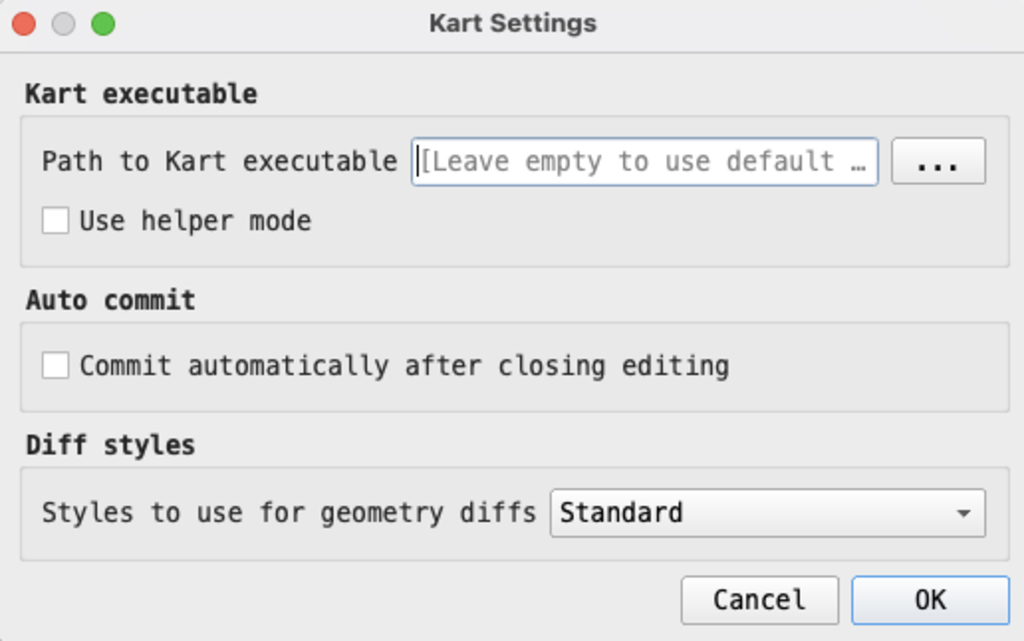
\includegraphics{img/kart-settings.png}
\end{center}

\subsubsection{Connect to a local
repository}\label{connect-to-a-local-repository}

If a side panel has not already appeared, click on \emph{Plugins
\textgreater{} Kart \textgreater{} Repositories} to open the kart panel.
The panel will look empty, but we will populate it with the repository
we created before.

\begin{center}
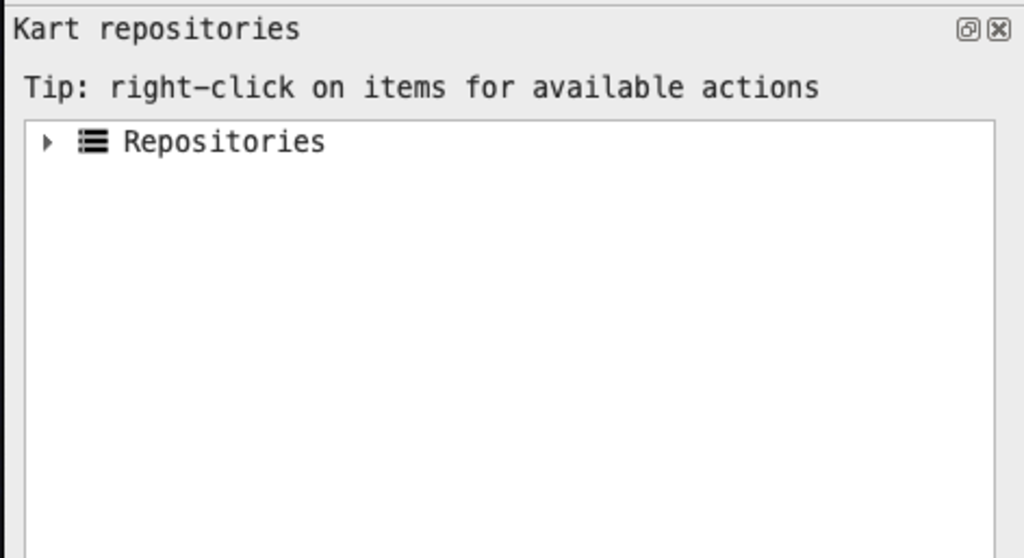
\includegraphics{img/kart-panel.png}
\end{center}

In order to do so, right click on ``Repositories''. You will see a list
of options: the last two (\emph{Create new repository} and \emph{Clone
repository}) are graphical replacement to the steps we did before
(Section~\ref{sec-kart-empty} and Section~\ref{sec-clone-repo}).

Click on \emph{Add existing repository\ldots{}} and navigate to the
\emph{kart-workflow} folder we created before, then click on ``Open''.

\begin{center}
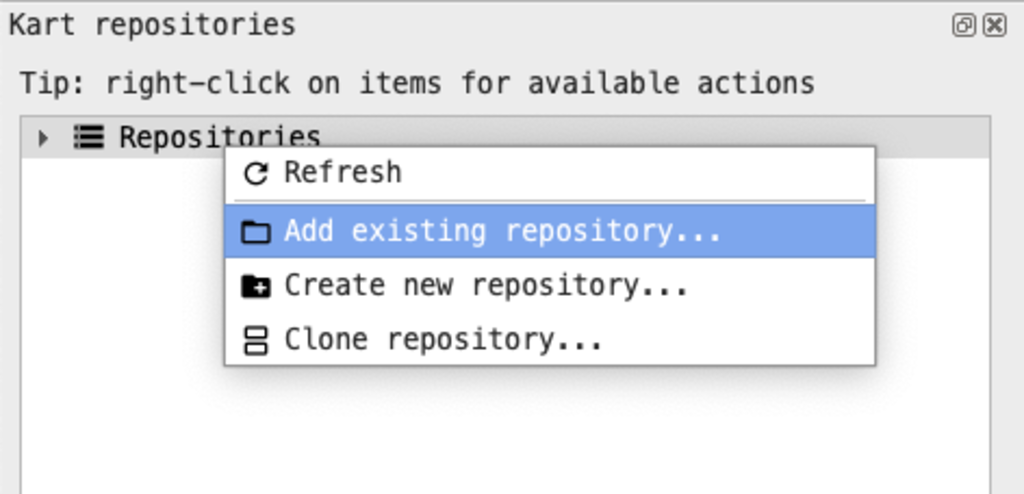
\includegraphics{img/kart-panel-right-click.png}
\end{center}

You will see the repository path now listed inside the panel under the
name \texttt{path/kart-workflow/kart-tutorial\ {[}main{]}}. The
\texttt{{[}main{]}} bit indicates the branch on which we are working
(just as the git branches, more on this on the
\href{https://docs.kartproject.org/en/latest/pages/quick_guide.html\#branching}{kart
documentation} and below in Section~\ref{sec-branching}).

\begin{center}
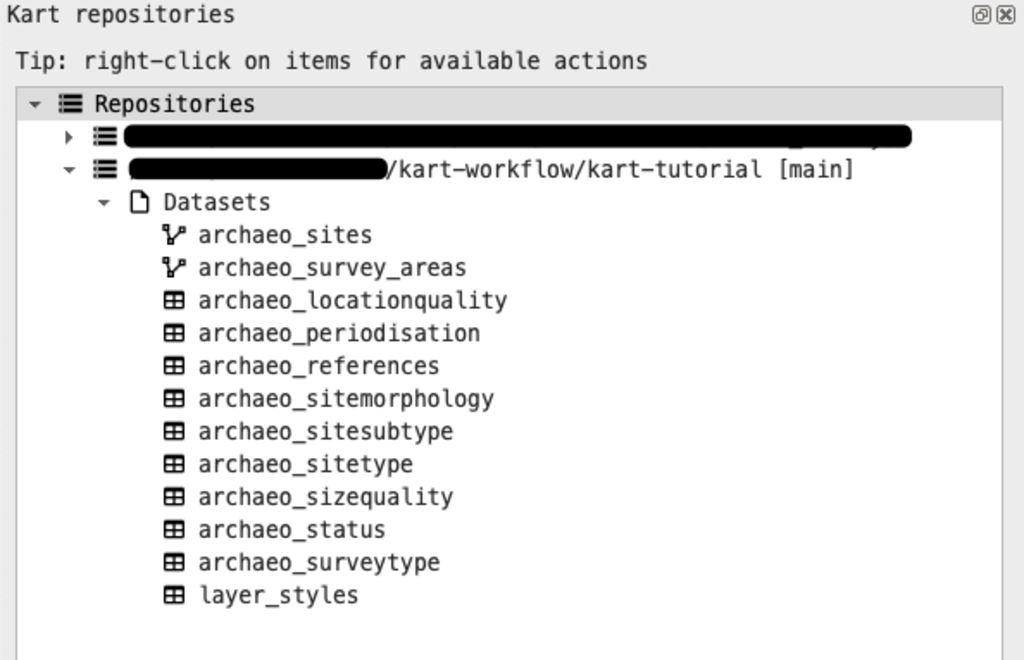
\includegraphics{img/kart-panel-expand.png}
\end{center}

\begin{tcolorbox}[enhanced jigsaw, bottomrule=.15mm, opacitybacktitle=0.6, colback=white, toptitle=1mm, left=2mm, titlerule=0mm, leftrule=.75mm, title={Tip}, opacityback=0, colframe=quarto-callout-tip-color-frame, breakable, colbacktitle=quarto-callout-tip-color!10!white, coltitle=black, bottomtitle=1mm, toprule=.15mm, arc=.35mm, rightrule=.15mm]

For more information on the data, see the Appendix or our
\href{https://github.com/UnitoAssyrianGovernance/.github/wiki/GIS-Vector-Data\#main-layer-table-structure}{wiki
section}.

\end{tcolorbox}

\subsubsection{Load data inside the
project}\label{load-data-inside-the-project}

What you connected to is what kart calls
\href{https://docs.kartproject.org/en/latest/pages/quick_guide.html\#workflow}{working
copy}, i.e.~a file living on your computer that you can interact with
through GIS. Kart uses different
\href{https://docs.kartproject.org/en/latest/pages/wc_types.html}{working
copy types}, in our case the
\href{https://docs.kartproject.org/en/latest/pages/wc_types/gpkg_wc.html}{Geopackage
working copy}.

To add the layers to our QGIS project, expand the repository tree by
clicking on the arrow button on the left in the kart panel. Right-click
on the \texttt{archaeo\_sites} layer and click on \emph{Add to QGIS
Project}. A point layer should appear on the map and the CRS should
change to EPSG:32636. Add also all the other layers (you should have 10
tabular layer and another 1 geometry layer. Add \ul{all of them} except
the \texttt{layer\_styles} layer. These table layer are background data
useful for populating records in the main layer (archaeo\_sites) through
\href{https://docs.qgis.org/3.34/en/docs/user_manual/working_with_vector/vector_properties.html\#edit-widgets}{QGIS
value relation widgets}.

\begin{center}
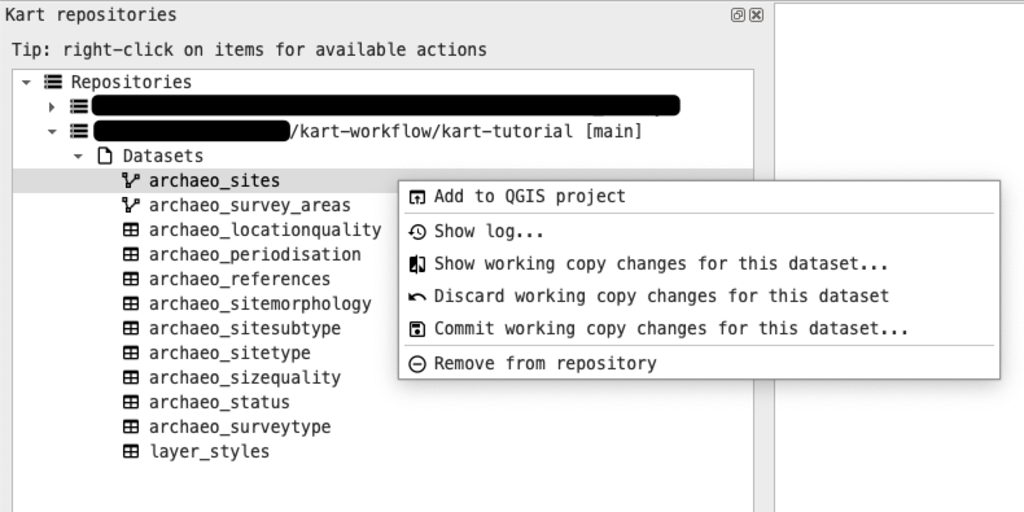
\includegraphics{img/kart-panel-add-project.png}
\end{center}

\subsubsection{Add new geometry to existing layers}\label{sec-add-geom}

You can now proceed to add new data as you would do normally in QGIS.
Toggle the editing for the \texttt{archaeo\_sites} layer and click on
the \emph{Add Point Feature} button. Click anywhere and add a new point.
Fill the attribute table however you like. The tab structure you will
see in the new feature prompt is thank to
\href{https://docs.qgis.org/3.34/en/docs/user_manual/working_with_vector/vector_properties.html\#attributes-form-properties}{QGIS
attribute form feature}, and because the style of the layer is saved
inside the geopackage, and versioned in kart as well (this was the
\texttt{layer\_styles} layer present in the repository listing in the
kart panel.

\begin{center}
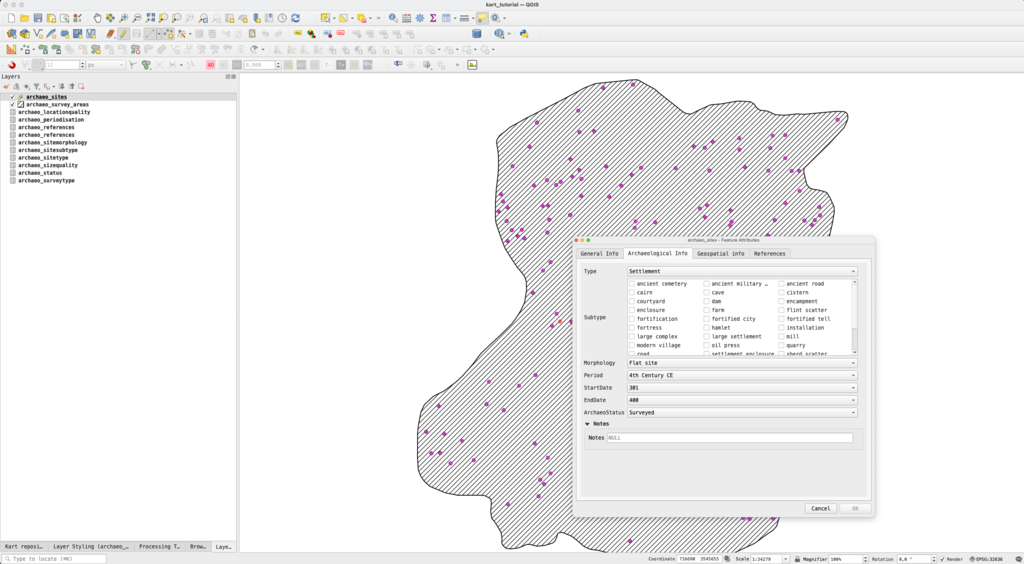
\includegraphics{img/qgis-add-new-feature.png}
\end{center}

Save the edits by either closing the editing tool or clicking on the
\emph{Save Layer Edits} button.

\subsubsection{Edit an existing
geometry}\label{edit-an-existing-geometry}

Let's edit an existing point now, for example by changing its position
and modifying some attributes. Use the
\href{https://docs.qgis.org/3.34/en/docs/user_manual/introduction/general_tools.html\#identify}{identify
features tool} to quickly access the attribute table of a point of your
choice, and right click on the identify panel to bring up a contextual
menu. From this menu select \emph{Edit Feature Form}. Edit the attribute
table, e.g.~changing the site type or the periodization, and saving your
edits.

\begin{center}
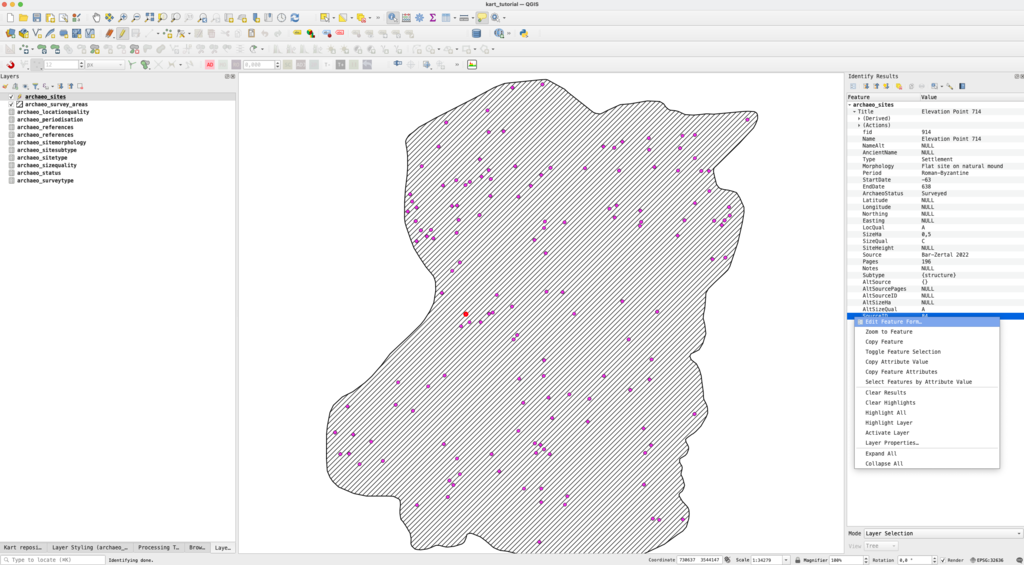
\includegraphics{img/qgis-identify-attr-table.png}
\end{center}

\begin{center}
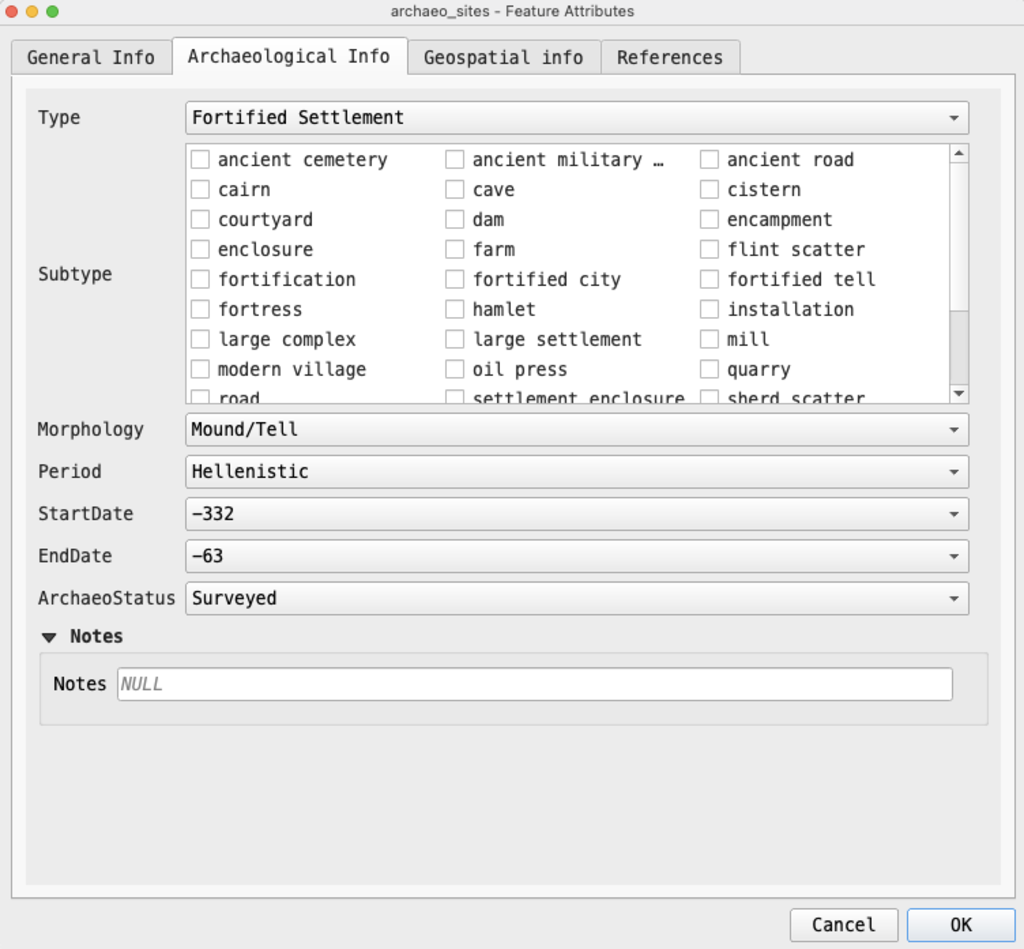
\includegraphics{img/qgis-attr-table.png}
\end{center}

Now let's also change the location of one of the points. It can either
be the same one or another, but for an easier visualization later, it
might be best to edit points near the one we added before. Use the move
feature tool to do it and move a point a bit further from its actual
location, saving the edits after.

\begin{center}
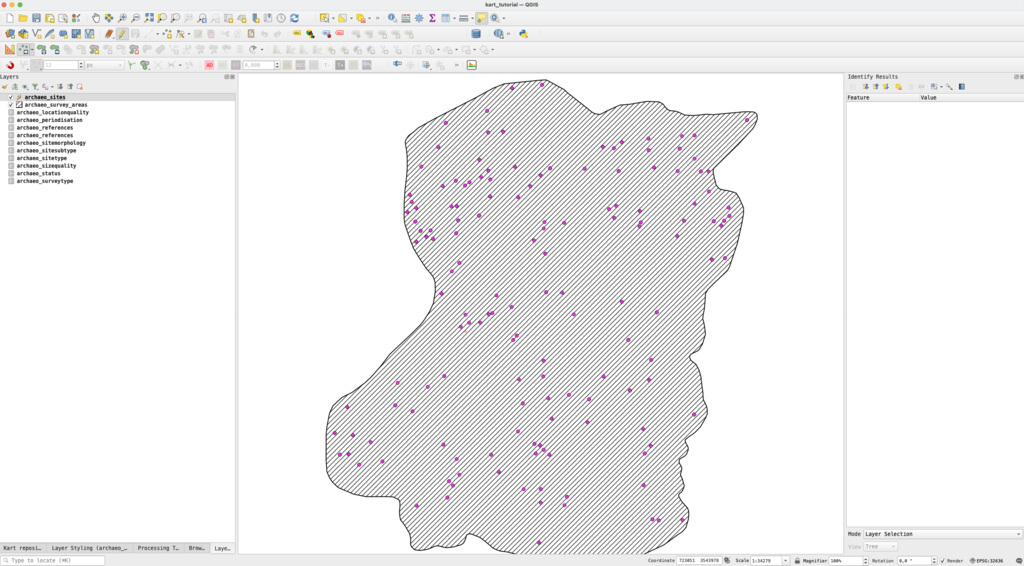
\includegraphics{img/qgis-move-feature.png}
\end{center}

\subsubsection{Inspect working copy
changes}\label{inspect-working-copy-changes}

One of the interesting aspects of Kart is the possibility of inspecting
changes before commits. The QGIS plugin in particular offers a way of
graphically visualize changes, both on a 2D map or in a table layout. To
do so, return to the kart repository panel and right-click on the
repository name, then click on the \emph{Show working copy
changes\ldots{}} button (you can also right-click on a single layer to
inspect changes only for that one).

\begin{center}
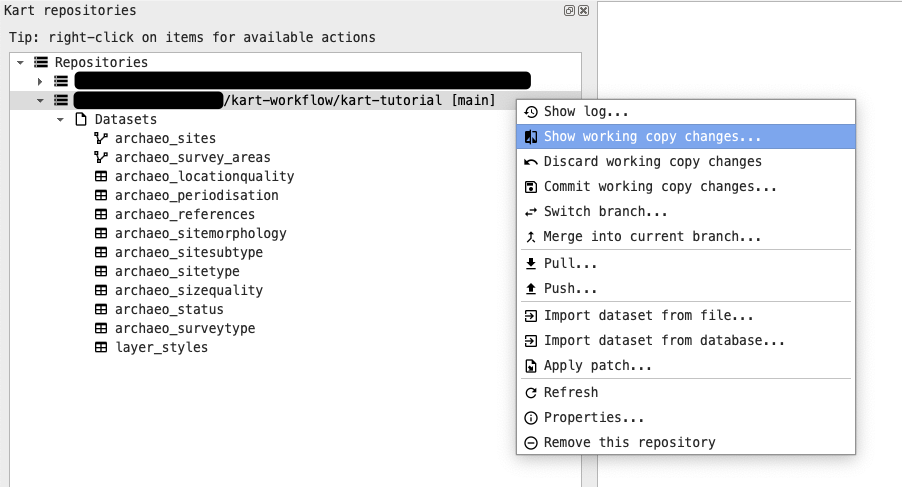
\includegraphics{img/kart-panel-show-wc-changes.png}
\end{center}

The visual diff viewer panel will open. On the left we can see (in a
tree-like structure) the layer that was edited (archaeo\_sites, there
would be more if we had edited more than one layer), the type of change
(Added, Modified)m and the primary key of the added/modified entry. On
the right, there are two types of diffs available, the Attributes table,
and the Geometries tab. For the Added feature, the attribute table will
be all green (as these are all new entries), and the geometry tab will
not be much useful. However, if we switch to the \emph{Modified}
features, we can see that kart highlights the rows that have been
modified in a convenient table with Old/New value pairs.

\begin{center}
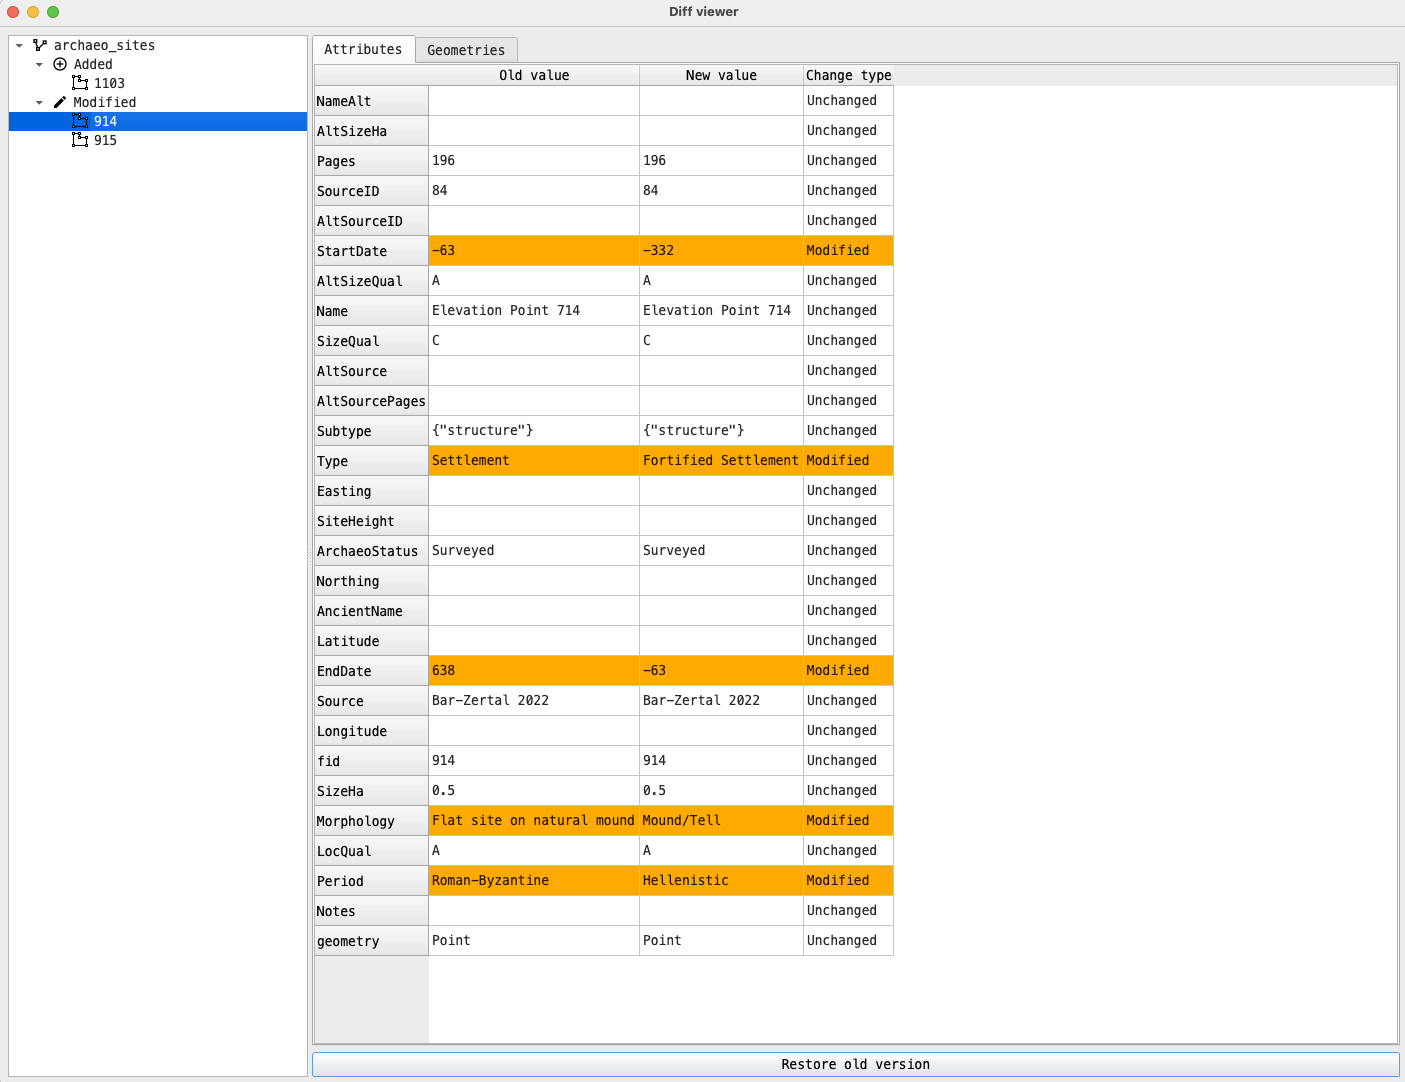
\includegraphics{img/kart-diff-attributes.png}
\end{center}

If we switch to the Geometries tab instead, and select the point that we
have moved from the list on the left, then we will see how Kart
highlights with transparency the previous location of the geometry/nodes
and in a darker color the new location.

On the top of the Geometries tab, there are also two dropdown dialogs,
one (\emph{Additional Layers}) related to the layer we want to show in
the Diff Viewer \ul{in addition to the modified geometries} (options
are: Project Layer, OSM Basemap, No additional layers), and another
(\emph{Diff type}) related to how we want to visualize the Diff (options
are: Transparency, Swipe, Per-vertex diff). We found both transparency
and per-vertex diff to be particularly useful in case of polygon
geometries.

\begin{center}
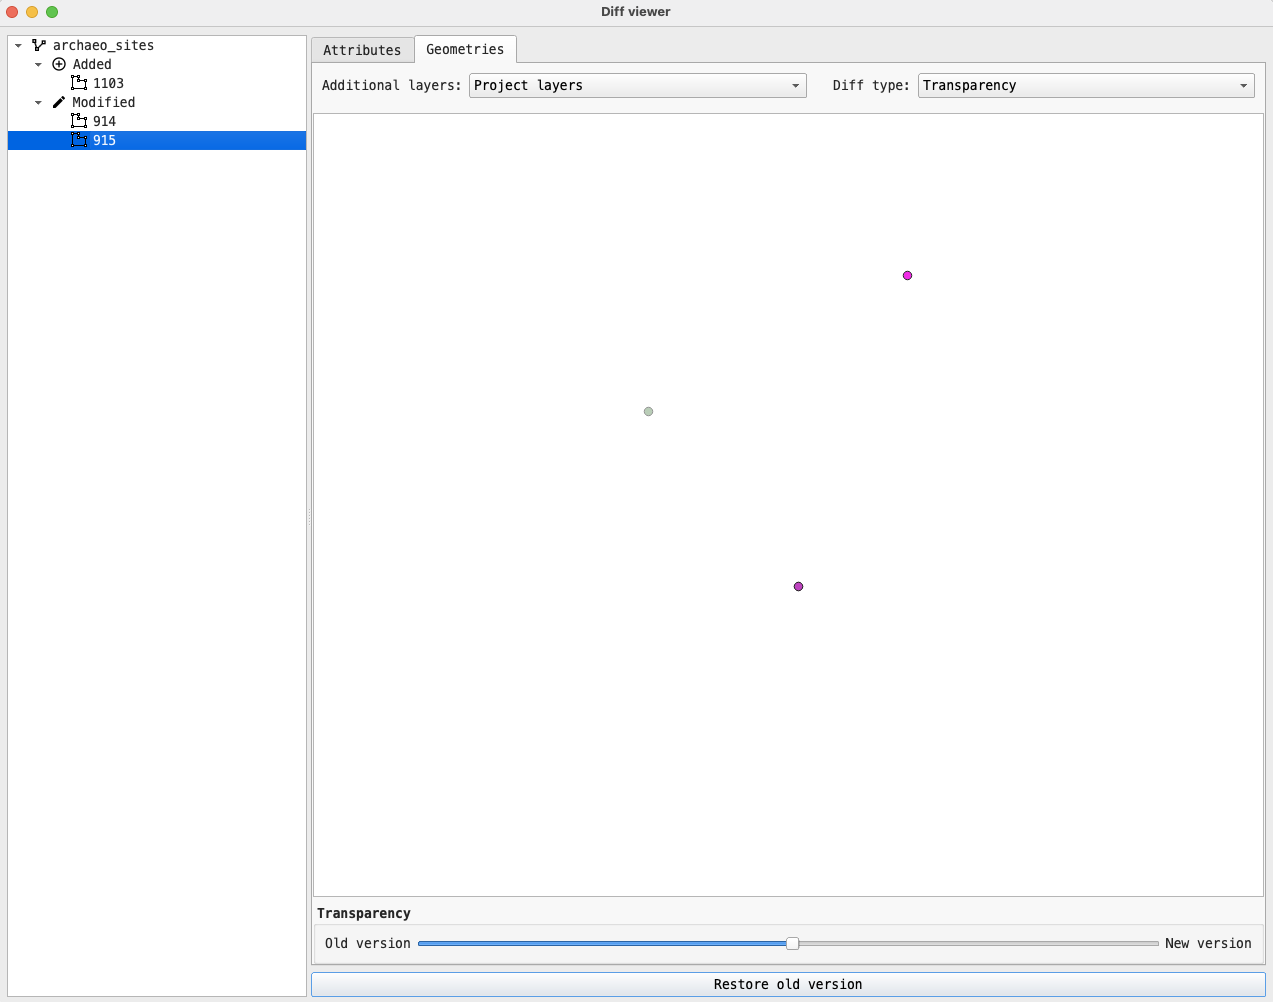
\includegraphics{img/kart-diff-geometry.png}
\end{center}

Note that the kart CLI also offers a way to inspect changes to the
working copy, through the \texttt{kart\ status} and \texttt{kart\ diff}
\href{https://docs.kartproject.org/en/latest/pages/basic_usage_tutorial.html\#making-and-committing-changes}{commands}.
For example, for the edits that we just made the output would be
something similar:

\begin{tcolorbox}[enhanced jigsaw, bottomrule=.15mm, opacitybacktitle=0.6, colback=white, toptitle=1mm, left=2mm, titlerule=0mm, leftrule=.75mm, title={Expand}, opacityback=0, colframe=quarto-callout-note-color-frame, breakable, colbacktitle=quarto-callout-note-color!10!white, coltitle=black, bottomtitle=1mm, toprule=.15mm, arc=.35mm, rightrule=.15mm]

\begin{Shaded}
\begin{Highlighting}[]
\ExtensionTok{kart}\NormalTok{ status}
\ExtensionTok{On}\NormalTok{ branch main}

\ExtensionTok{Changes}\NormalTok{ in working copy:}
  \KeywordTok{(}\ExtensionTok{use} \StringTok{"kart commit"}\NormalTok{ to commit}\KeywordTok{)}
  \KeywordTok{(}\ExtensionTok{use} \StringTok{"kart restore"}\NormalTok{ to discard changes}\KeywordTok{)}

  \ExtensionTok{archaeo\_sites:}
    \ExtensionTok{feature:}
      \ExtensionTok{1}\NormalTok{ inserts}
      \ExtensionTok{1}\NormalTok{ updates}

\ExtensionTok{kart}\NormalTok{ diff}
\ExtensionTok{{-}{-}{-}}\NormalTok{ archaeo\_sites:feature:914}
\ExtensionTok{+++}\NormalTok{ archaeo\_sites:feature:914}
\ExtensionTok{{-}}\NormalTok{                                     Type = Settlement}
\ExtensionTok{+}\NormalTok{                                     Type = Fortified Settlement}
\ExtensionTok{{-}}\NormalTok{                               Morphology = Flat site on natural mound}
\ExtensionTok{+}\NormalTok{                               Morphology = Mound/Tell}
\ExtensionTok{{-}}\NormalTok{                                   Period = Roman{-}Byzantine}
\ExtensionTok{+}\NormalTok{                                   Period = Hellenistic}
\ExtensionTok{{-}}\NormalTok{                                StartDate = }\AttributeTok{{-}63}
\ExtensionTok{+}\NormalTok{                                StartDate = }\AttributeTok{{-}332}
\ExtensionTok{{-}}\NormalTok{                                  EndDate = 638}
\ExtensionTok{+}\NormalTok{                                  EndDate = }\AttributeTok{{-}63}
\ExtensionTok{+++}\NormalTok{ archaeo\_sites:feature:1103}
\ExtensionTok{+}\NormalTok{                                      fid = 1103}
\ExtensionTok{+}\NormalTok{                                 geometry = POINT}\ErrorTok{(}\ExtensionTok{...}\KeywordTok{)}
\ExtensionTok{+}\NormalTok{                                     Name = A new point}
\ExtensionTok{+}\NormalTok{                                  NameAlt = ␀}
\ExtensionTok{+}\NormalTok{                              AncientName = ␀}
\ExtensionTok{+}\NormalTok{                                     Type = Settlement}
\ExtensionTok{+}\NormalTok{                               Morphology = Flat site}
\ExtensionTok{+}\NormalTok{                                   Period = Hellenistic}
\ExtensionTok{+}\NormalTok{                                StartDate = }\AttributeTok{{-}332}
\ExtensionTok{+}\NormalTok{                                  EndDate = }\AttributeTok{{-}63}
\ExtensionTok{+}\NormalTok{                            ArchaeoStatus = Surveyed}
\ExtensionTok{+}\NormalTok{                                 Latitude = ␀}
\ExtensionTok{+}\NormalTok{                                Longitude = ␀}
\ExtensionTok{+}\NormalTok{                                 Northing = ␀}
\ExtensionTok{+}\NormalTok{                                  Easting = ␀}
\ExtensionTok{+}\NormalTok{                                  LocQual = A}
\ExtensionTok{+}\NormalTok{                                   SizeHa = ␀}
\ExtensionTok{+}\NormalTok{                                 SizeQual = C}
\ExtensionTok{+}\NormalTok{                               SiteHeight = ␀}
\ExtensionTok{+}\NormalTok{                                   Source = Archaeological Survey of Israel}
\ExtensionTok{+}\NormalTok{                                    Pages = ␀}
\ExtensionTok{+}\NormalTok{                                    Notes = ␀}
\ExtensionTok{+}\NormalTok{                                  Subtype = \{}\StringTok{"hamlet"}\NormalTok{\}}
\ExtensionTok{+}\NormalTok{                                AltSource = ␀}
\ExtensionTok{+}\NormalTok{                           AltSourcePages = ␀}
\ExtensionTok{+}\NormalTok{                              AltSourceID = ␀}
\ExtensionTok{+}\NormalTok{                                AltSizeHa = ␀}
\ExtensionTok{+}\NormalTok{                              AltSizeQual = ␀}
\ExtensionTok{+}\NormalTok{                                 SourceID = 1kart status}
\end{Highlighting}
\end{Shaded}

\end{tcolorbox}

\subsubsection{Commit working copy
changes}\label{commit-working-copy-changes}

Now that we inspected the changes made during editing, we can commit
them, just like git. In QGIS, go back to the kart repositories panel and
right-click on our repository, then select \emph{Commit working copy
changes\ldots{}} (you can also discard them if you noticed some errors).
A dialog will pop-up prompting you to enter a commit message. Write a
descriptive commit message and then click on ``Ok''. A green message at
the top should inform you that the changes have been committed
successfully (Changes correctly commited).

\begin{center}
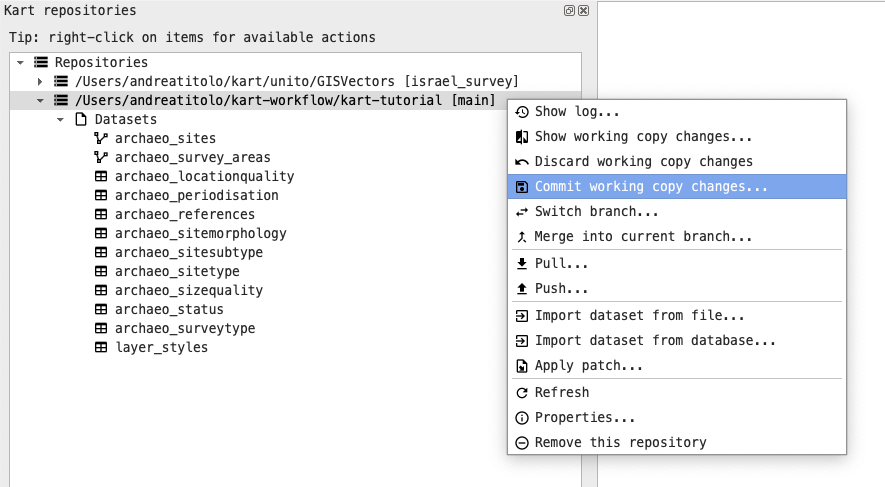
\includegraphics{img/kart-panel-commit.png}
\end{center}

You can achieve the same by using the CLI through the command
\texttt{kart\ commit}
(\href{https://docs.kartproject.org/en/latest/pages/command_reference.html\#commit-changes-to-a-working-copy}{relevant
documentation}).

\begin{Shaded}
\begin{Highlighting}[]
\ExtensionTok{kart}\NormalTok{ commit }\AttributeTok{{-}m} \StringTok{\textquotesingle{}YOUR COMMIT MESSAGE\textquotesingle{}}
\ExtensionTok{[main}\NormalTok{ be39e89] your commit message}
  \ExtensionTok{archaeo\_sites:}
    \ExtensionTok{feature:}
      \ExtensionTok{1}\NormalTok{ inserts}
      \ExtensionTok{2}\NormalTok{ updates}
  \ExtensionTok{Date:}\NormalTok{ Wed Apr 10 16:40:04 2024 +0200}
\end{Highlighting}
\end{Shaded}

\begin{tcolorbox}[enhanced jigsaw, bottomrule=.15mm, opacitybacktitle=0.6, colback=white, toptitle=1mm, left=2mm, titlerule=0mm, leftrule=.75mm, title=\textcolor{quarto-callout-tip-color}{\faLightbulb}\hspace{0.5em}{Before proceeding}, opacityback=0, colframe=quarto-callout-tip-color-frame, breakable, colbacktitle=quarto-callout-tip-color!10!white, coltitle=black, bottomtitle=1mm, toprule=.15mm, arc=.35mm, rightrule=.15mm]

Add a couple more points or modify existing ones, and make at least
other two-three commits, by repeating the same steps above. You can also
edit different layers, such has the table layers, or the survey\_areas
layers.

\end{tcolorbox}

\subsubsection{Inspect the commit tree}\label{inspect-the-commit-tree}

Now that we have more than just a couple of commits, we can use the
visual log to inspect commits to our main branch. To access the log,
right-click on our repository in the kart panel and click on \emph{Show
log\ldots{}}

The log panel will appear (if you have worked with VSCode or any other
editor providing a git-tree functionality, this will look very
familiar). For now it will look rather simple as we are directly
committing on a single branch and we have few commits. The corresponding
command for the CLI is \texttt{kart\ log} (note: if you are using pagers
for git, these will not work with kart of course)

\begin{center}
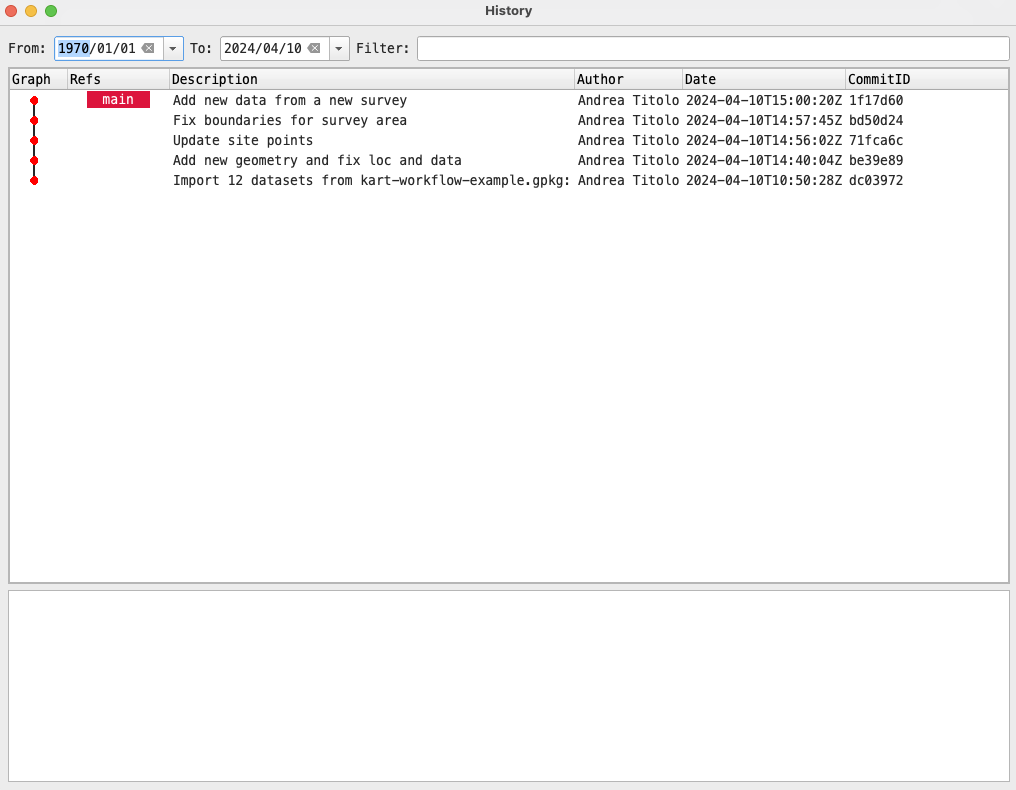
\includegraphics{img/kart-log.png}
\end{center}

\subsubsection{Inspect changes introduced in a specific commit (and
other
options)}\label{inspect-changes-introduced-in-a-specific-commit-and-other-options}

In the QGIS plugin, we can inspect, using the Visual Diff tool, changes
introduced by each commit we made. We can bring up a contextual menu by
right-clicking on a commit, and a number of options will show. We will
not inspect all the options visible in the image below, but they should
be self-explanatory, especially if you are familiar with git.

\begin{center}
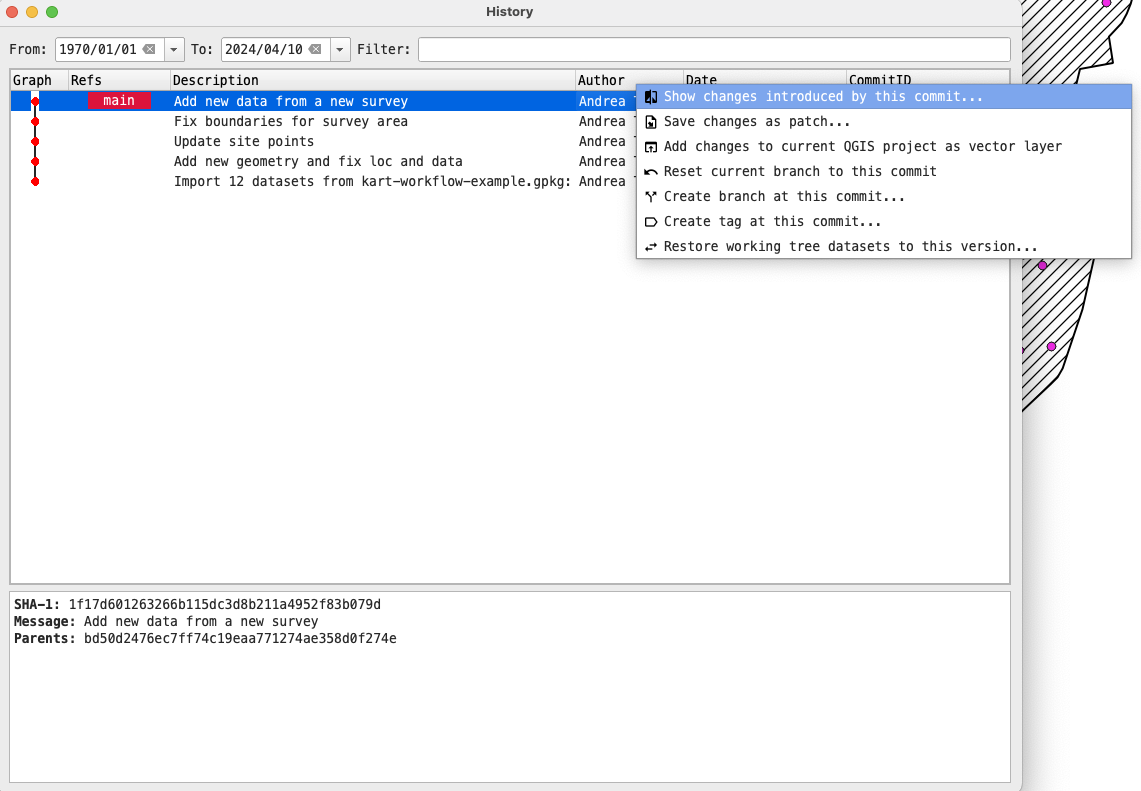
\includegraphics{img/kart-log-right-click.png}
\end{center}

\subsection{Collaborating with Kart}\label{sec-collaboration}

While kart is perfectly usable on a local machine only, the goal here is
to collaborate with other people. In our workflow, every person can make
edits to the layers that need to be worked on. Git is, in general, a
very good collaboration tool, and thus kart potentially offers similar
advantages. We will explore a very simple worklow: we will simulate one
colleague creating a secondary branch from \texttt{main}, adds the edits
needed, and then merge back into \texttt{main}, where another colleague
have already added geometries to the same layers. Since we are using a
geopackage, we will have to deal with conflicts, so we will explore that
too.

\begin{tcolorbox}[enhanced jigsaw, bottomrule=.15mm, opacitybacktitle=0.6, colback=white, toptitle=1mm, left=2mm, titlerule=0mm, leftrule=.75mm, title=\textcolor{quarto-callout-caution-color}{\faFire}\hspace{0.5em}{Warning}, opacityback=0, colframe=quarto-callout-caution-color-frame, breakable, colbacktitle=quarto-callout-caution-color!10!white, coltitle=black, bottomtitle=1mm, toprule=.15mm, arc=.35mm, rightrule=.15mm]

Here we are using the \texttt{main} branch as an example to avoid too
much redundancy, but this is usually \textbf{not a good practice}, as
usually is best to have everyone working on secondary branches. As
suggested in
\href{https://github.com/koordinates/kart/issues/814\#issuecomment-1498167436}{this
comment}, it is recommended that one user will do the merge, push the
changes, and any other user will use the merged branch as starting point
for any new edits in order to avoid further conflicts. This means that
after the merge into main is completed and the updated main has been
pushed to remote, new edits \textbf{should be done on new branches
created from the updated main branch} (after updating the local main
branch with \texttt{kart\ pull}).

\end{tcolorbox}

\subsubsection{Branching}\label{sec-branching}

Branching is a common way to implement features and changes isolated
from the main working tree and from other people working on the same
dataset. The \texttt{main} branch is the default branch upon repository
creation.

In order to create a new branch, you can use the graphical plugin by
right-clicking on the repository name and then click on \emph{Switch
branch..} On the the new dialog click on \emph{Create New}. In the new
dialog pop-up select the name of the new branch (e.g.~\texttt{dev}) and
then click on \emph{OK}.

\begin{center}
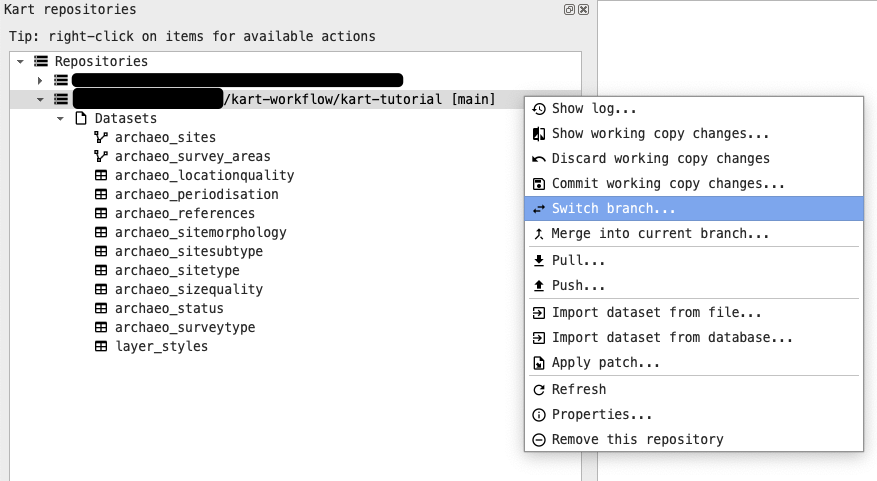
\includegraphics{img/kart-panel-branch.png}
\end{center}

\begin{center}
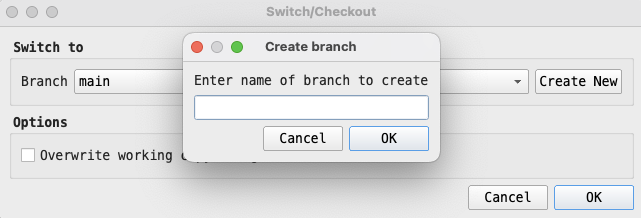
\includegraphics{img/kart-panel-switch-new.png}
\end{center}

You can reproduce the exact same behavior with less clicks using the
following command in your terminal when in the kart repo:
\texttt{kart\ checkout\ -b\ dev}.

Your worktree will switch to the new branch automatically. If you need
to switch back to \texttt{main} again, from the plugin panel use the
same \emph{Switch branch..} option and select \texttt{main} from the
dropdown menu. From the CLI you can use \texttt{kart\ switch\ main} or
\texttt{kart\ checkout\ main}.

If you use the CLI, the changes should be immediately visible in the
plugin panel in QGIS, if that's not the case, you can refresh using
\texttt{F5} or by right-clicking on the repo and click \emph{Refresh}.

You can also see the two branches (at the same point in the kart tree)
using the \emph{Show log..} button from the kart repo panel.

\begin{center}
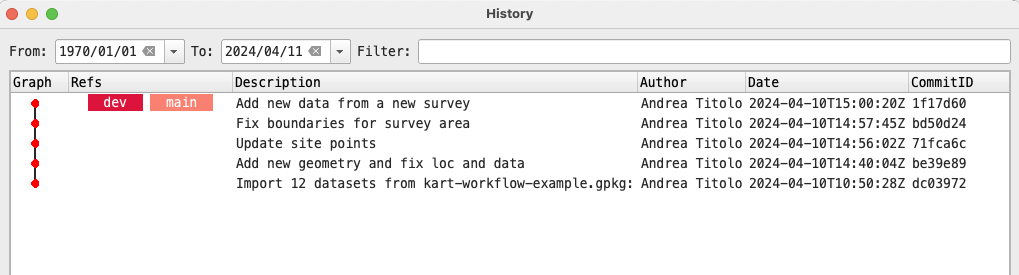
\includegraphics{img/kart-panel-branches-log.png}
\end{center}

\begin{quote}
For more general information about branches: see the
\href{https://github.com/koordinates/kart-qgis-plugin/blob/main/docs/index.md\#working-with-branches}{Kart
QGIS Plugin docs} and the
\href{https://docs.kartproject.org/en/latest/pages/quick_guide.html\#branching}{Kart
docs} and
\href{https://docs.kartproject.org/en/latest/pages/command_reference.html\#branching-and-merging}{command
reference}.
\end{quote}

\paragraph{Add features on the new
branch}\label{add-features-on-the-new-branch}

Let's now add 3 new points to the \emph{archaeo\_sites} layer while on
the \texttt{dev} branch. The procedure is the same as the one
highlighted in the previous sections (Section~\ref{sec-add-geom}). Let's
also commit this changes and inspect the worktree to see that the
\texttt{dev} branch is now ahead of \texttt{main} by 1 commit.

\begin{center}
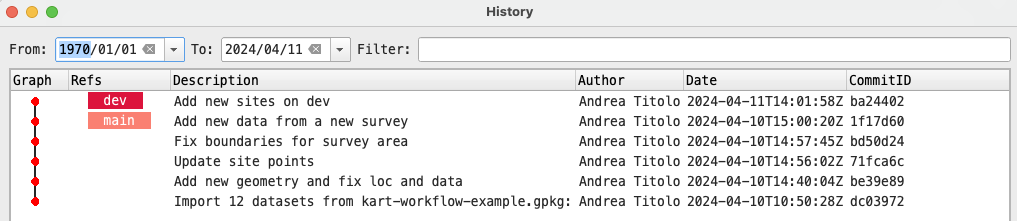
\includegraphics{img/kart-panel-dev-branch-ahead.png}
\end{center}

\paragraph{Add features to the main
branch}\label{add-features-to-the-main-branch}

To simulate a collaborative situation, switch back to the \texttt{main}
branch (using the plugin interface of \texttt{kart\ switch}) and add 2
points to the same \emph{archaeo\_sites} layer and commit our changes.

\subsubsection{Merging}\label{sec-merging}

We want our changes on the \texttt{dev} branch to be incorporated on the
\texttt{main} branch. To do this we can use the graphical plugin to
start a merge. While on the \texttt{main} branch, right-click on the
repository and select \emph{Merge into current branch..} In the new
panel you can provide a merge message and select other options, but for
now let's just make sure to select \texttt{dev} from the dropdown
corresponding to \textbf{Branch.}

You can do the same in the terminal by using \texttt{kart\ merge\ dev},
make sure you are on the \texttt{main} branch.

If there are no conflicts, kart will merge using the fast-forward
option(thus we will not find a ``merge'' commit in your commit history)
and our branch main will be updated with the edits from the other
branch. However, this is not the case now.

If you did like we did above, you will likely see a message telling you
that there were conflicts during the merge, and that these conflicts
need to be resolved before continuing with the merge.

\begin{center}
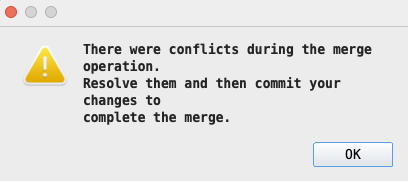
\includegraphics{img/kart-panel-conflicts.png}
\end{center}

If you use the command line, you will receive a similar message:

\begin{Shaded}
\begin{Highlighting}[]
\ExtensionTok{kart}\NormalTok{ merge dev}

\ExtensionTok{Merging}\NormalTok{ branch }\StringTok{"dev"}\NormalTok{ into main}
\ExtensionTok{Conflicts}\NormalTok{ found:}

\ExtensionTok{archaeo\_sites:}
    \ExtensionTok{archaeo\_sites:feature:}\NormalTok{ 2 conflicts}

\ExtensionTok{Repository}\NormalTok{ is now in }\StringTok{"merging"}\NormalTok{ state.}
\ExtensionTok{View}\NormalTok{ conflicts with }\KeywordTok{\textasciigrave{}}\ExtensionTok{kart}\NormalTok{ conflicts}\KeywordTok{\textasciigrave{}}\NormalTok{ and resolve them with }\KeywordTok{\textasciigrave{}}\ExtensionTok{kart}\NormalTok{ resolve}\KeywordTok{\textasciigrave{}}\NormalTok{.}
\ExtensionTok{Once}\NormalTok{ no conflicts remain, complete this merge with }\KeywordTok{\textasciigrave{}}\ExtensionTok{kart}\NormalTok{ merge }\AttributeTok{{-}{-}continue}\KeywordTok{\textasciigrave{}}\NormalTok{.}
\ExtensionTok{Or}\NormalTok{ use }\KeywordTok{\textasciigrave{}}\ExtensionTok{kart}\NormalTok{ merge }\AttributeTok{{-}{-}abort}\KeywordTok{\textasciigrave{}}\NormalTok{ to return to the previous state.}
\end{Highlighting}
\end{Shaded}

\subsubsection{Dealing with conflicts}\label{sec-conflicts}

When conflicts are encountered, the repository enters into a
\textbf{merging} state. In this state no changes can be made to the
dataset until the conflicts are resolved. Three options are available to
us:

\begin{enumerate}
\def\labelenumi{\arabic{enumi}.}
\tightlist
\item
  Solve the conflicts
\item
  Continue merge (this will not work until conflicts are solved)
\item
  Abort the merge (return to the previous state before the merge
  command)
\end{enumerate}

We want to solve our conflicts. When working with geopackages, the most
likely conflict comes from conflicting primary keys (in the \texttt{fid}
field).

\paragraph{Viewing conflicts}\label{viewing-conflicts}

To solve our conflicts we need first to see what is actually
conflicting. With the QGIS plugin, right click on the repository and
select \emph{Resolve conflicts\ldots{}}

\begin{tcolorbox}[enhanced jigsaw, bottomrule=.15mm, opacitybacktitle=0.6, colback=white, toptitle=1mm, left=2mm, titlerule=0mm, leftrule=.75mm, title=\textcolor{quarto-callout-note-color}{\faInfo}\hspace{0.5em}{Note}, opacityback=0, colframe=quarto-callout-note-color-frame, breakable, colbacktitle=quarto-callout-note-color!10!white, coltitle=black, bottomtitle=1mm, toprule=.15mm, arc=.35mm, rightrule=.15mm]

Currently we are unable to access the graphical tool due to a possible
bug in kart, thus we will continue with the CLI only. We will update
this tutorial with the relevant info once we get past this issue. If you
don't want to use the CLI, you can try following the
\href{https://github.com/koordinates/kart-qgis-plugin/blob/main/docs/index.md\#working-with-branches}{kart
plugin docs} about solving conflicts and then continue on to the next
section.

\end{tcolorbox}

To see the conflicts on the CLI, use \texttt{kart\ conflicts} to
generate a list of conflicting features. While not immediately
noticeable, you will see that each feature has a \texttt{:ours} or
\texttt{:theirs} after its name, indicating at which branch they
pertain, \texttt{ours} meaning the branch you are currently on, and
\texttt{theirs} meaning the branch you are mergin from. In our case,
ours is \texttt{main} and theirs is yourbranchname (or how your feature
branch is called). This view does not really tell you which fields are
conflicting, but if you look at the \texttt{fid} you will see that they
are duplicated.

\begin{tcolorbox}[enhanced jigsaw, bottomrule=.15mm, opacitybacktitle=0.6, colback=white, toptitle=1mm, left=2mm, titlerule=0mm, leftrule=.75mm, title={Expand}, opacityback=0, colframe=quarto-callout-note-color-frame, breakable, colbacktitle=quarto-callout-note-color!10!white, coltitle=black, bottomtitle=1mm, toprule=.15mm, arc=.35mm, rightrule=.15mm]

\begin{Shaded}
\begin{Highlighting}[]
\ExtensionTok{kart}\NormalTok{ conflicts}
\ExtensionTok{archaeo\_sites:}
    \ExtensionTok{archaeo\_sites:feature:}
        \ExtensionTok{archaeo\_sites:feature:1106:}
            \ExtensionTok{archaeo\_sites:feature:1106:ours:}
                                     \ExtensionTok{fid}\NormalTok{ = 1106}
                                \ExtensionTok{geometry}\NormalTok{ = POINT}\ErrorTok{(}\ExtensionTok{...}\KeywordTok{)}
                                    \ExtensionTok{Name}\NormalTok{ = A site on main branch}
                                 \ExtensionTok{NameAlt}\NormalTok{ = ␀}
                             \ExtensionTok{AncientName}\NormalTok{ = ␀}
                                    \ExtensionTok{Type}\NormalTok{ = Building}
                              \ExtensionTok{Morphology}\NormalTok{ = Flat site}
                                  \ExtensionTok{Period}\NormalTok{ = Roman}
                               \ExtensionTok{StartDate}\NormalTok{ = }\AttributeTok{{-}63}
                                 \ExtensionTok{EndDate}\NormalTok{ = 324}
                           \ExtensionTok{ArchaeoStatus}\NormalTok{ = Surveyed}
                                \ExtensionTok{Latitude}\NormalTok{ = ␀}
                               \ExtensionTok{Longitude}\NormalTok{ = ␀}
                                \ExtensionTok{Northing}\NormalTok{ = ␀}
                                 \ExtensionTok{Easting}\NormalTok{ = ␀}
                                 \ExtensionTok{LocQual}\NormalTok{ = A}
                                  \ExtensionTok{SizeHa}\NormalTok{ = ␀}
                                \ExtensionTok{SizeQual}\NormalTok{ = C}
                              \ExtensionTok{SiteHeight}\NormalTok{ = ␀}
                                  \ExtensionTok{Source}\NormalTok{ = kart4arch2024}
                                   \ExtensionTok{Pages}\NormalTok{ = ␀}
                                   \ExtensionTok{Notes}\NormalTok{ = ␀}
                                 \ExtensionTok{Subtype}\NormalTok{ = \{}\StringTok{"farm"}\NormalTok{\}}
                               \ExtensionTok{AltSource}\NormalTok{ = ␀}
                          \ExtensionTok{AltSourcePages}\NormalTok{ = ␀}
                             \ExtensionTok{AltSourceID}\NormalTok{ = ␀}
                               \ExtensionTok{AltSizeHa}\NormalTok{ = ␀}
                             \ExtensionTok{AltSizeQual}\NormalTok{ = ␀}
                                \ExtensionTok{SourceID}\NormalTok{ = 3}
            \ExtensionTok{archaeo\_sites:feature:1106:theirs:}
                                     \ExtensionTok{fid}\NormalTok{ = 1106}
                                \ExtensionTok{geometry}\NormalTok{ = POINT}\ErrorTok{(}\ExtensionTok{...}\KeywordTok{)}
                                    \ExtensionTok{Name}\NormalTok{ = A first site on dev}
                                 \ExtensionTok{NameAlt}\NormalTok{ = ␀}
                             \ExtensionTok{AncientName}\NormalTok{ = ␀}
                                    \ExtensionTok{Type}\NormalTok{ = Settlement}
                              \ExtensionTok{Morphology}\NormalTok{ = Flat site}
                                  \ExtensionTok{Period}\NormalTok{ = Late Bronze Age}
                               \ExtensionTok{StartDate}\NormalTok{ = }\AttributeTok{{-}1550}
                                 \ExtensionTok{EndDate}\NormalTok{ = }\AttributeTok{{-}1150}
                           \ExtensionTok{ArchaeoStatus}\NormalTok{ = Surveyed}
                                \ExtensionTok{Latitude}\NormalTok{ = ␀}
                               \ExtensionTok{Longitude}\NormalTok{ = ␀}
                                \ExtensionTok{Northing}\NormalTok{ = ␀}
                                 \ExtensionTok{Easting}\NormalTok{ = ␀}
                                 \ExtensionTok{LocQual}\NormalTok{ = A}
                                  \ExtensionTok{SizeHa}\NormalTok{ = ␀}
                                \ExtensionTok{SizeQual}\NormalTok{ = C}
                              \ExtensionTok{SiteHeight}\NormalTok{ = ␀}
                                  \ExtensionTok{Source}\NormalTok{ = kart4arch2024}
                                   \ExtensionTok{Pages}\NormalTok{ = ␀}
                                   \ExtensionTok{Notes}\NormalTok{ = ␀}
                                 \ExtensionTok{Subtype}\NormalTok{ = \{}\StringTok{"farm"}\NormalTok{\}}
                               \ExtensionTok{AltSource}\NormalTok{ = ␀}
                          \ExtensionTok{AltSourcePages}\NormalTok{ = ␀}
                             \ExtensionTok{AltSourceID}\NormalTok{ = ␀}
                               \ExtensionTok{AltSizeHa}\NormalTok{ = ␀}
                             \ExtensionTok{AltSizeQual}\NormalTok{ = ␀}
                                \ExtensionTok{SourceID}\NormalTok{ = 5}
        \ExtensionTok{archaeo\_sites:feature:1107:}
            \ExtensionTok{archaeo\_sites:feature:1107:ours:}
                                     \ExtensionTok{fid}\NormalTok{ = 1107}
                                \ExtensionTok{geometry}\NormalTok{ = POINT}\ErrorTok{(}\ExtensionTok{...}\KeywordTok{)}
                                    \ExtensionTok{Name}\NormalTok{ = Another site on main branch}
                                 \ExtensionTok{NameAlt}\NormalTok{ = ␀}
                             \ExtensionTok{AncientName}\NormalTok{ = ␀}
                                    \ExtensionTok{Type}\NormalTok{ = Settlement}
                              \ExtensionTok{Morphology}\NormalTok{ = Flat site on natural mound}
                                  \ExtensionTok{Period}\NormalTok{ = Byzantine}
                               \ExtensionTok{StartDate}\NormalTok{ = 324}
                                 \ExtensionTok{EndDate}\NormalTok{ = 638}
                           \ExtensionTok{ArchaeoStatus}\NormalTok{ = Surveyed}
                                \ExtensionTok{Latitude}\NormalTok{ = ␀}
                               \ExtensionTok{Longitude}\NormalTok{ = ␀}
                                \ExtensionTok{Northing}\NormalTok{ = ␀}
                                 \ExtensionTok{Easting}\NormalTok{ = ␀}
                                 \ExtensionTok{LocQual}\NormalTok{ = A}
                                  \ExtensionTok{SizeHa}\NormalTok{ = ␀}
                                \ExtensionTok{SizeQual}\NormalTok{ = C}
                              \ExtensionTok{SiteHeight}\NormalTok{ = ␀}
                                  \ExtensionTok{Source}\NormalTok{ = kart4arch2024}
                                   \ExtensionTok{Pages}\NormalTok{ = ␀}
                                   \ExtensionTok{Notes}\NormalTok{ = ␀}
                                 \ExtensionTok{Subtype}\NormalTok{ = \{}\StringTok{"hamlet"}\NormalTok{\}}
                               \ExtensionTok{AltSource}\NormalTok{ = ␀}
                          \ExtensionTok{AltSourcePages}\NormalTok{ = ␀}
                             \ExtensionTok{AltSourceID}\NormalTok{ = ␀}
                               \ExtensionTok{AltSizeHa}\NormalTok{ = ␀}
                             \ExtensionTok{AltSizeQual}\NormalTok{ = ␀}
                                \ExtensionTok{SourceID}\NormalTok{ = 4}
            \ExtensionTok{archaeo\_sites:feature:1107:theirs:}
                                     \ExtensionTok{fid}\NormalTok{ = 1107}
                                \ExtensionTok{geometry}\NormalTok{ = POINT}\ErrorTok{(}\ExtensionTok{...}\KeywordTok{)}
                                    \ExtensionTok{Name}\NormalTok{ = A second site on dev}
                                 \ExtensionTok{NameAlt}\NormalTok{ = ␀}
                             \ExtensionTok{AncientName}\NormalTok{ = ␀}
                                    \ExtensionTok{Type}\NormalTok{ = Fortified Settlement}
                              \ExtensionTok{Morphology}\NormalTok{ = Mound/Tell}
                                  \ExtensionTok{Period}\NormalTok{ = Iron Age II}
                               \ExtensionTok{StartDate}\NormalTok{ = }\AttributeTok{{-}950}
                                 \ExtensionTok{EndDate}\NormalTok{ = }\AttributeTok{{-}586}
                           \ExtensionTok{ArchaeoStatus}\NormalTok{ = Surveyed}
                                \ExtensionTok{Latitude}\NormalTok{ = ␀}
                               \ExtensionTok{Longitude}\NormalTok{ = ␀}
                                \ExtensionTok{Northing}\NormalTok{ = ␀}
                                 \ExtensionTok{Easting}\NormalTok{ = ␀}
                                 \ExtensionTok{LocQual}\NormalTok{ = A}
                                  \ExtensionTok{SizeHa}\NormalTok{ = ␀}
                                \ExtensionTok{SizeQual}\NormalTok{ = C}
                              \ExtensionTok{SiteHeight}\NormalTok{ = ␀}
                                  \ExtensionTok{Source}\NormalTok{ = kart4arch2024}
                                   \ExtensionTok{Pages}\NormalTok{ = ␀}
                                   \ExtensionTok{Notes}\NormalTok{ = ␀}
                                 \ExtensionTok{Subtype}\NormalTok{ = \{}\StringTok{"fortification"}\NormalTok{\}}
                               \ExtensionTok{AltSource}\NormalTok{ = ␀}
                          \ExtensionTok{AltSourcePages}\NormalTok{ = ␀}
                             \ExtensionTok{AltSourceID}\NormalTok{ = ␀}
                               \ExtensionTok{AltSizeHa}\NormalTok{ = ␀}
                             \ExtensionTok{AltSizeQual}\NormalTok{ = ␀}
                                \ExtensionTok{SourceID}\NormalTok{ = 6}
\end{Highlighting}
\end{Shaded}

\end{tcolorbox}

\paragraph{Solving conflicts}\label{solving-conflicts}

We need now to resolve the conflicts. In git you will be thrown in the
text editor, but kart lets us choose the way in which to resolve it.
However, the way indicated on the official documentation
(\href{https://docs.kartproject.org/en/latest/pages/command_reference.html\#resolving-a-conflict}{\texttt{kart\ revolve\ -\/-with=(ancestors\textbar{}ours\textbar{}theirs\textbar{}delete)}})
does not include, at the time of writing (2023-12-06) the most suitable
option, i.e.~automatically renumbering the features. This is instead
only documented on a
\href{https://github.com/koordinates/kart/pull/817}{pull request}, so we
report it here too (note that however the option is visible in the
\emph{man page} using \texttt{kart\ resolve\ -\/-help)}.

Since Kart version
\href{https://github.com/koordinates/kart/releases/tag/v0.12.3}{0.12.3},
there is a \texttt{kart\ revolve\ -\/-renumber=(ours\textbar{}theirs)}
command that is intended to automatically resolve primary key conflicts
during merge operations. The \texttt{-\/-renumber} flag takes one of the
two options: \texttt{ours} or \texttt{theirs}, with ours meaning the
branch we are currently on, and theirs meaning the branch we are merging
from.

Let's use \texttt{kart\ resolve\ -\/-renumber=theirs} or \texttt{ours}
by typing the command in our terminal.

We suggest using \texttt{theirs} as to preserve the order of features
originally present in the main branch, but feel free to use
\texttt{ours} if you prefer (see below).

\begin{tcolorbox}[enhanced jigsaw, bottomrule=.15mm, opacitybacktitle=0.6, colback=white, toptitle=1mm, left=2mm, titlerule=0mm, leftrule=.75mm, title=\textcolor{quarto-callout-important-color}{\faExclamation}\hspace{0.5em}{Caution}, opacityback=0, colframe=quarto-callout-important-color-frame, breakable, colbacktitle=quarto-callout-important-color!10!white, coltitle=black, bottomtitle=1mm, toprule=.15mm, arc=.35mm, rightrule=.15mm]

If there is only a partial overlapping of primary keys, kart will merge
those keys that can be merged, while the other features will wait for
the conflict resolution to be renumbered. This means that if you have
some keys in the \texttt{yourbranchname} branch that do not overlap with
primary keys in your \texttt{main} branch, and you use \texttt{theirs}
as an option for renumbering, these primary keys will be added first
after the keys already present in \texttt{main} (as mentioned
\href{https://github.com/koordinates/kart/pull/817}{here}). This will
break the sequential order of features from the secondary branch,
however, it is more of a visual issue than a real one, unless you are
relying on the order of those primary keys for other operations.

\end{tcolorbox}

After running the command, you should see something like this:

\begin{Shaded}
\begin{Highlighting}[]
\ExtensionTok{kart}\NormalTok{ resolve }\AttributeTok{{-}{-}renumber}\OperatorTok{=}\NormalTok{theirs}
\ExtensionTok{Resolved}\NormalTok{ 2 conflicts. 0 conflicts to go.}
\ExtensionTok{Use} \KeywordTok{\textasciigrave{}}\ExtensionTok{kart}\NormalTok{ merge }\AttributeTok{{-}{-}continue}\KeywordTok{\textasciigrave{}}\NormalTok{ to complete the merge}
\end{Highlighting}
\end{Shaded}

As adivides by the CLI, let's run \texttt{kart\ merge\ -\/-continue} to
finish the merge (this can be done also in the graphical plugin).

\subparagraph{A note about terminal text
editors}\label{sec-text-editors}

By default, you will be prompted to insert a commit message inside a
terminal text editor. Which text editor this will be is dependent on
your machine, OS, and configuration. If you have set the
\texttt{\$VISUAL} or \texttt{\$EDITOR} variables in your shell, then you
will know what will be opened. If not, you will either be put inside
nano/emacs or vi/vim.

\begin{tcolorbox}[enhanced jigsaw, bottomrule=.15mm, opacitybacktitle=0.6, colback=white, toptitle=1mm, left=2mm, titlerule=0mm, leftrule=.75mm, title={With some possible differences, the interface will be like this for
vi/vim}, opacityback=0, colframe=quarto-callout-note-color-frame, breakable, colbacktitle=quarto-callout-note-color!10!white, coltitle=black, bottomtitle=1mm, toprule=.15mm, arc=.35mm, rightrule=.15mm]

\begin{figure}[H]

{\centering 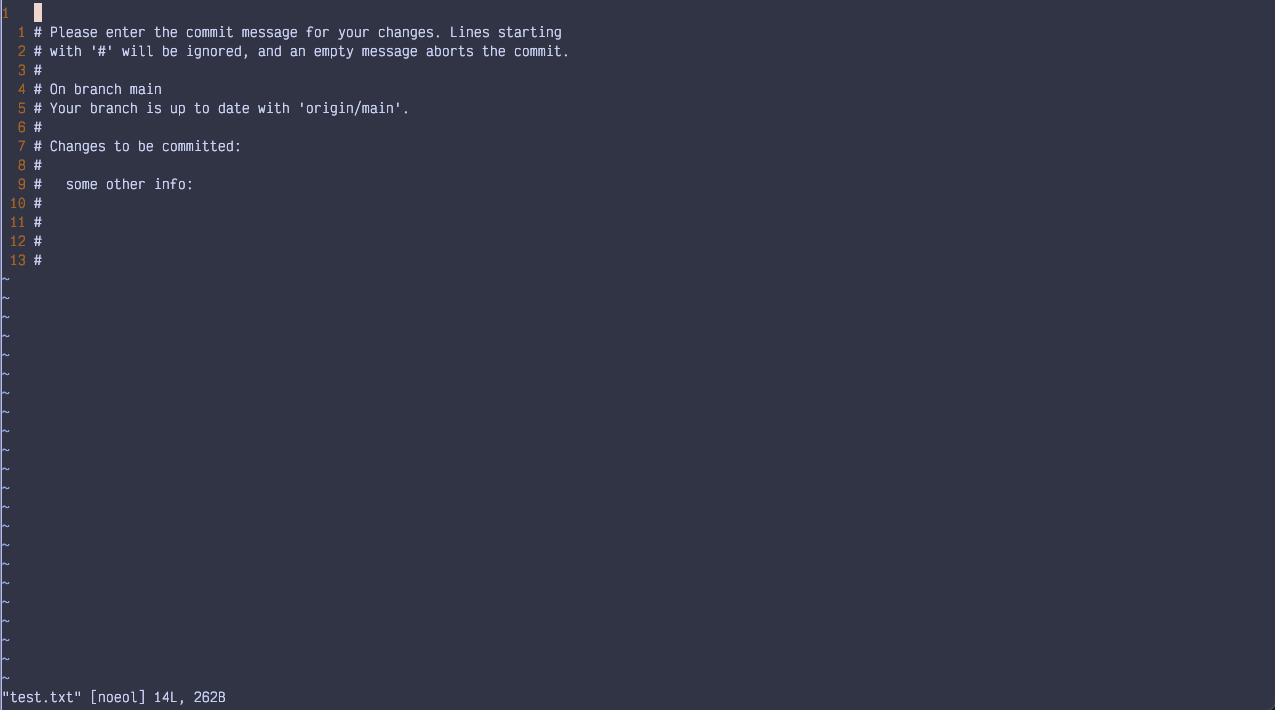
\includegraphics{img/vi_interface.png}

}

\caption{vi/vim interface}

\end{figure}%

\end{tcolorbox}

\begin{tcolorbox}[enhanced jigsaw, bottomrule=.15mm, opacitybacktitle=0.6, colback=white, toptitle=1mm, left=2mm, titlerule=0mm, leftrule=.75mm, title={And like this for nano/emacs:}, opacityback=0, colframe=quarto-callout-note-color-frame, breakable, colbacktitle=quarto-callout-note-color!10!white, coltitle=black, bottomtitle=1mm, toprule=.15mm, arc=.35mm, rightrule=.15mm]

\begin{figure}[H]

{\centering 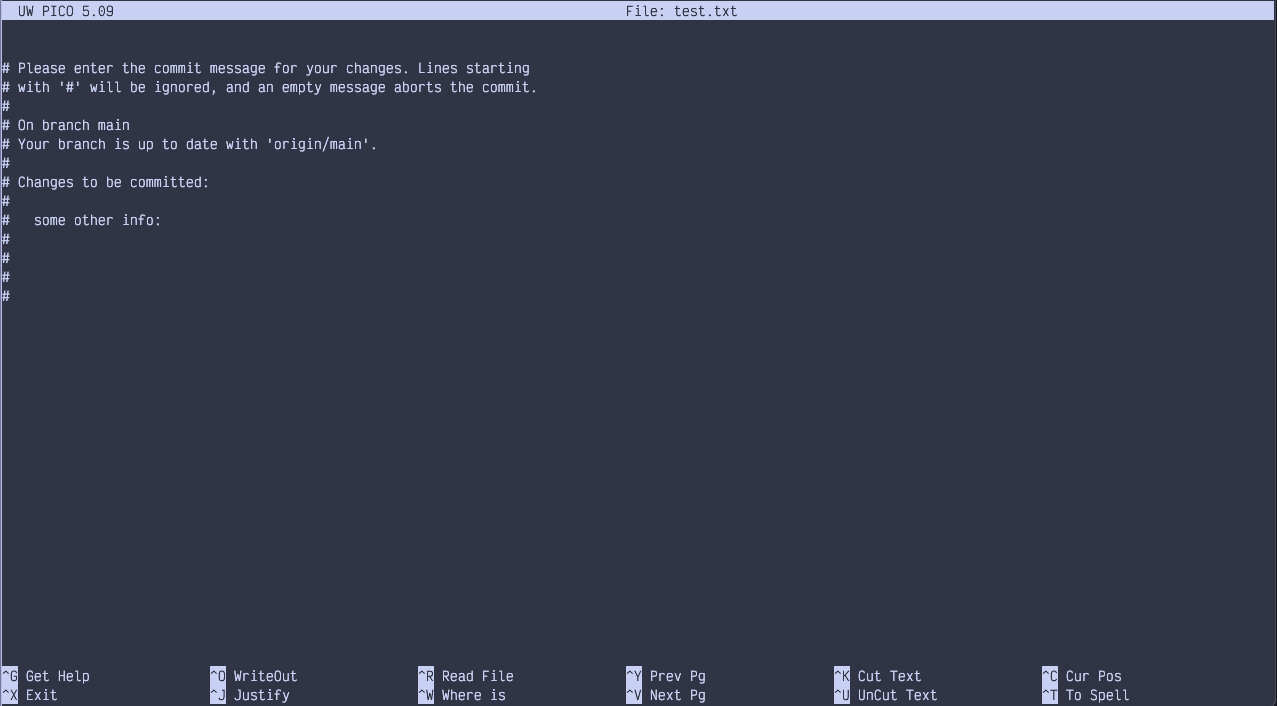
\includegraphics{img/nano_interface.png}

}

\caption{nano/emacs interface}

\end{figure}%

\end{tcolorbox}

You will already have a commit message written for you, something like
\texttt{Merge\ branch\ "dev"\ into\ main}. You can edit the message (see
below) or accept the defaul by using \texttt{ctrl+x} in nano/emacs or
\texttt{:wq} in vi/vim.

To edit the message in nano, start typing at the top of the top of the
file. When you are finished, the menu at the bottom should tell you how
to quit and save. Press ctrl+x (the \texttt{\^{}} means ctrl) to exit.
When asked to save the buffer, press \texttt{y} to confirm.

To edit the message in vi/vim, press \texttt{i} to be able to type (this
might not be necessary). Type the commit message and when satisfied
press \texttt{:q} to exit (typing \texttt{:q!} will exit without saving
the file).

The text editor will close and the terminal will output the details of
the commit and the date, plus some other info.

If everything went well you will see a message like this:

\begin{Shaded}
\begin{Highlighting}[]
\ExtensionTok{Merging}\NormalTok{ branch }\StringTok{"dev"}\NormalTok{ into main}
\ExtensionTok{No}\NormalTok{ conflicts!}
\ExtensionTok{Merge}\NormalTok{ committed as 890e2455fe81f0e58c5c5bed8cb7010e4fb174f8}
\ExtensionTok{Updating}\NormalTok{ kart{-}tutorial.gpkg ..}
\end{Highlighting}
\end{Shaded}

And your repo will be available to edit again. Check the features and
you will see that the \texttt{main} branch now includes also the ones
from \texttt{dev}.

You can inspect the worktree to see how the branches diverged and how
the merge commit was created.

\begin{center}
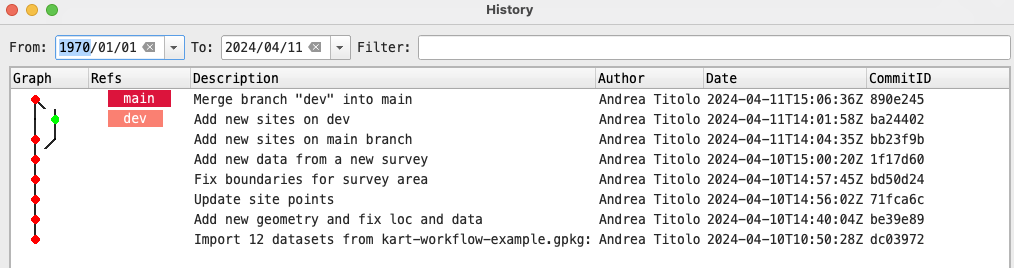
\includegraphics{img/kart-panel-merge-result.png}
\end{center}

\begin{quote}
See also
\href{https://github.com/koordinates/kart-qgis-plugin/blob/main/docs/index.md\#working-with-branches}{Kart
QGIS plugin docs} and
\href{https://docs.kartproject.org/en/latest/pages/command_reference.html\#resolving-conflicts}{Kart
docs} on resolving conflicts and
our\href{https://github.com/UnitoAssyrianGovernance/.github/wiki/GIS-Vector-Data\#dealing-with-conflicts}{Wiki
on the same topic}. A useful
\href{https://github.com/koordinates/kart/issues/814}{github issue}
about solving conflicts in multi-user scenario.
\end{quote}

\paragraph{Delete branches}\label{delete-branches}

Now that we have merged the features, we can safely delete the
\texttt{dev} branch to clean our kart repository. To our knowledge this
option is still not available through the graphical plugin.

\begin{tcolorbox}[enhanced jigsaw, bottomrule=.15mm, opacitybacktitle=0.6, colback=white, toptitle=1mm, left=2mm, titlerule=0mm, leftrule=.75mm, title={Note}, opacityback=0, colframe=quarto-callout-note-color-frame, breakable, colbacktitle=quarto-callout-note-color!10!white, coltitle=black, bottomtitle=1mm, toprule=.15mm, arc=.35mm, rightrule=.15mm]

You cannot delete the branch you are currently on, so you will need to
switch to another branch in order to delete it.

\end{tcolorbox}

To delete a branch you can use this command
\texttt{kart\ branch\ -d\ dev} (the \texttt{d} flag stands for
\emph{delete}).

You should see a confirmation message:

\begin{Shaded}
\begin{Highlighting}[]
\ExtensionTok{Deleted}\NormalTok{ branch dev }\ErrorTok{(}\ExtensionTok{was}\NormalTok{ ba24402}\KeywordTok{)}\BuiltInTok{.}
\end{Highlighting}
\end{Shaded}

And you can confirm there is only one branch by running
\texttt{kart\ branch\ -v} in the terminal:

\begin{Shaded}
\begin{Highlighting}[]
\ExtensionTok{kart}\NormalTok{ branch }\AttributeTok{{-}a}
\ExtensionTok{*}\NormalTok{ main}
\end{Highlighting}
\end{Shaded}

\begin{tcolorbox}[enhanced jigsaw, bottomrule=.15mm, opacitybacktitle=0.6, colback=white, toptitle=1mm, left=2mm, titlerule=0mm, leftrule=.75mm, title=\textcolor{quarto-callout-important-color}{\faExclamation}\hspace{0.5em}{Important}, opacityback=0, colframe=quarto-callout-important-color-frame, breakable, colbacktitle=quarto-callout-important-color!10!white, coltitle=black, bottomtitle=1mm, toprule=.15mm, arc=.35mm, rightrule=.15mm]

If you do not delete you development branch, remember to start new works
by creating new branches from the \texttt{main} one, otherwise your
might branch from outdated dataset!

\end{tcolorbox}

\subsubsection{Push changes to a remote
repository}\label{push-changes-to-a-remote-repository}

Let's say you are finishing your work and you want to backup your data
outside of your machine, or you need to collaborate remotely with other
people, thus you need to use

\paragraph{Connect to a remote
repository}\label{connect-to-a-remote-repository}

Check that the repository has no remotes with
\texttt{kart\ remotes\ -v}.

If you cloned the repository in the initial steps
(Section~\ref{sec-clone-repo}), you might see some remotes (\ul{if you
don't, skip this part}):

\begin{Shaded}
\begin{Highlighting}[]
\ExtensionTok{kart}\NormalTok{ remote }\AttributeTok{{-}v}
\ExtensionTok{origin}\NormalTok{  https://github.com/UnitoAssyrianGovernance/kart{-}tutorial.git }\ErrorTok{(}\ExtensionTok{fetch}\KeywordTok{)}
\ExtensionTok{origin}\NormalTok{  https://github.com/UnitoAssyrianGovernance/kart{-}tutorial.git }\ErrorTok{(}\ExtensionTok{push}\KeywordTok{)}
\end{Highlighting}
\end{Shaded}

You will not be able to make push to these remotes, but to avoid
confusion remove these remotes from kart using the following:
\texttt{kart\ remote\ rm\ origin} (don't worry, this will not impact the
repository), and confirm again you have no more remotes using
\texttt{kart\ remotes\ -v}.

\subparagraph{Create a remote
repository}\label{create-a-remote-repository}

Create a remote repository on your forge of choice, in our case Github,
by following the respective
\href{https://docs.github.com/en/repositories/creating-and-managing-repositories/creating-a-new-repository}{instructions}.

\begin{tcolorbox}[enhanced jigsaw, bottomrule=.15mm, opacitybacktitle=0.6, colback=white, toptitle=1mm, left=2mm, titlerule=0mm, leftrule=.75mm, title=\textcolor{quarto-callout-warning-color}{\faExclamationTriangle}\hspace{0.5em}{Warning}, opacityback=0, colframe=quarto-callout-warning-color-frame, breakable, colbacktitle=quarto-callout-warning-color!10!white, coltitle=black, bottomtitle=1mm, toprule=.15mm, arc=.35mm, rightrule=.15mm]

As a general rule of thumb, if you are creating a repository from one
online forges, remember to NOT include any README.md, .gitignore, or
other files. Best-case scenario they will be ignored by kart, but
worst-case they might break your workflow, as kart will recognize an
out-of-sync remote with no real means of fixing it.

\end{tcolorbox}

\begin{center}
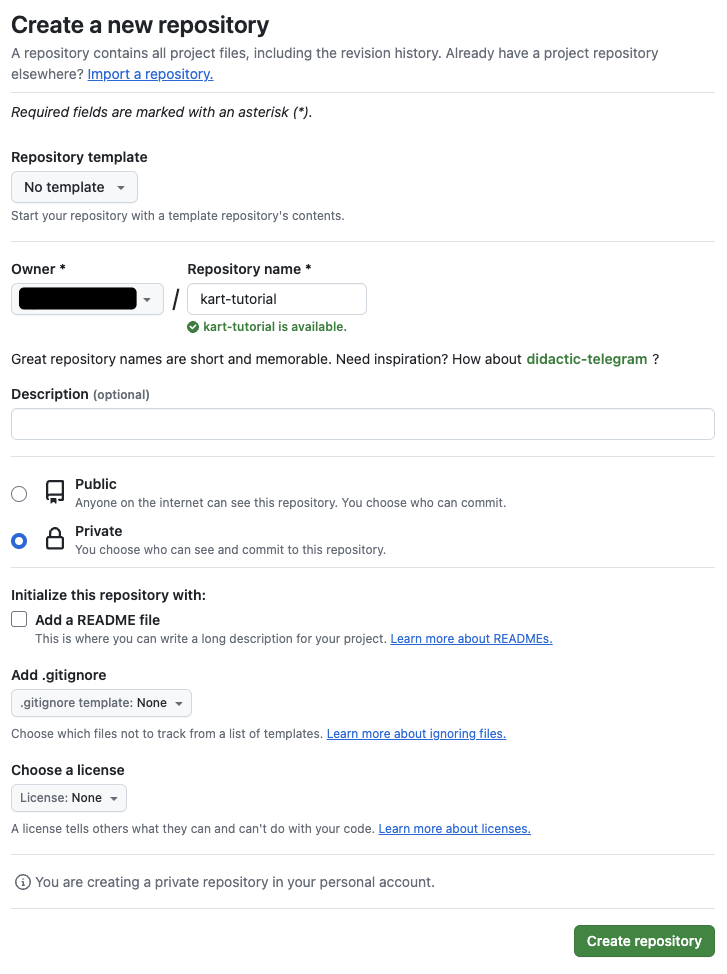
\includegraphics{img/github-create-repo.png}
\end{center}

\subparagraph{Connect with the kart QGIS
plugin}\label{connect-with-the-kart-qgis-plugin}

To connect to a remote repository through a graphical interface,
right-click on the repository panel and click on \emph{Push..}

\begin{center}
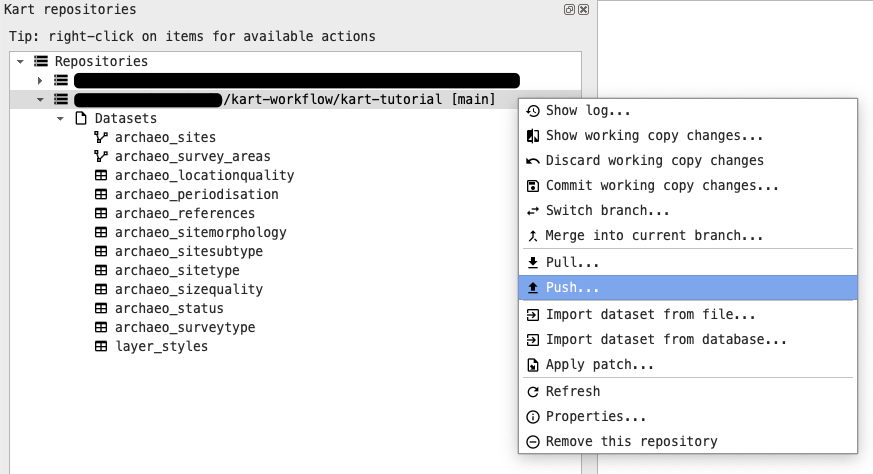
\includegraphics{img/kart-panel-push.png}
\end{center}

In the new dialog, click on \emph{Manage remotes}.

\begin{center}
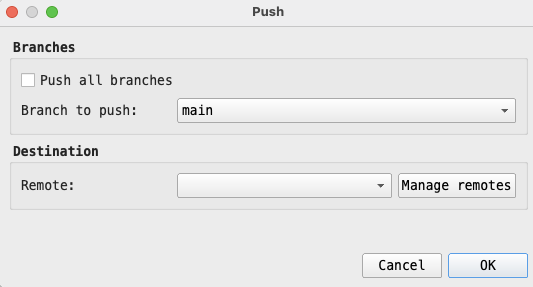
\includegraphics{img/kart-panel-push-manage.png}
\end{center}

In the new dialog, give a name to the Remote (e.g.~github or origin) and
the URL you will see after creating the new repository in the previous
steps. This URL will be something like
\texttt{https://github.com/yourusername/kart-tutorial.git} for HTTPS and
\texttt{git@github.com:\textasciigrave{}\textasciigrave{}yourusername\textasciigrave{}\textasciigrave{}/kart-tutorial.git}
for SSH (see above for HTTPS and SSH in Section~\ref{sec-https-ssh}).
After adding this information, click on \emph{Add New/Save} and then on
\emph{Ok} to close the dialog.

\begin{center}
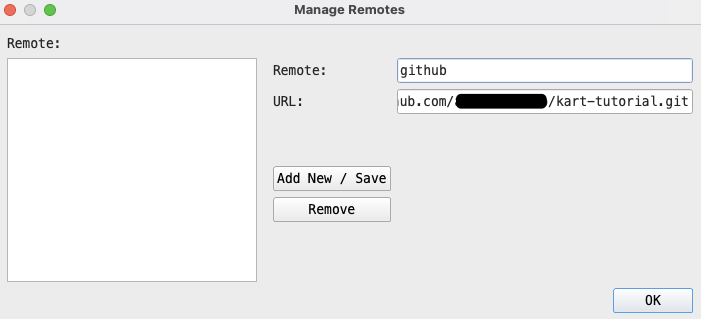
\includegraphics{img/kart-panel-remotes-add.png}
\end{center}

You will be back in the previous panel with the chosen remote added in
the dropdown (you can add more than one!).

\subparagraph{Connect with the kart
CLI}\label{connect-with-the-kart-cli}

To add a remote using the CLI, you can use
\texttt{kart\ remote\ add\ origin\ URL}, replacing the URL with the ones
mentioned above. Check if the remotes have been added using
\texttt{kart\ remotes\ -v} once again, you should see two entries with
your URL, one for fetch and one for push.

\begin{tcolorbox}[enhanced jigsaw, bottomrule=.15mm, opacitybacktitle=0.6, colback=white, toptitle=1mm, left=2mm, titlerule=0mm, leftrule=.75mm, title=\textcolor{quarto-callout-note-color}{\faInfo}\hspace{0.5em}{Note}, opacityback=0, colframe=quarto-callout-note-color-frame, breakable, colbacktitle=quarto-callout-note-color!10!white, coltitle=black, bottomtitle=1mm, toprule=.15mm, arc=.35mm, rightrule=.15mm]

\texttt{origin} is a convention, you can name your remote however you
want, just make sure to use the name you choose in the next commands.

\end{tcolorbox}

\paragraph{Push changes}\label{push-changes}

If you are using the graphical plugin, in the Push panel, click
\emph{Ok}. A green message should tell you that the push was successful.
If you encounter en error saying that the device is not configured, it
is likely an HTTPS authentication issue. You have some options:

\begin{enumerate}
\def\labelenumi{\arabic{enumi}.}
\tightlist
\item
  Make sure you are authenticated to github and that git has your
  credentials stored globally.
\item
  Use the CLI
\item
  Use SSH (which should be more reliable)
\end{enumerate}

\begin{quote}
Unfortunately the reason for an error might be a lot, if you encounter
some reach out to us and we will help as much as we can :)
\end{quote}

If you are using the CLI, run \texttt{kart\ push\ -u\ origin\ main}
(\textbf{origin is the name of the remote, change it accordingly}). If
you have not set your credentials before, you will be asked for your
forge username and token. If not, you will be able to push and you
should see something like this in your terminal:

\begin{Shaded}
\begin{Highlighting}[]
\ExtensionTok{kart}\NormalTok{ push }\AttributeTok{{-}u}\NormalTok{ origin main}

\ExtensionTok{Enumerating}\NormalTok{ objects: 892, done.}
\ExtensionTok{Counting}\NormalTok{ objects: 100\% }\ErrorTok{(}\ExtensionTok{892/892}\KeywordTok{)}\ExtensionTok{,}\NormalTok{ done.}
\ExtensionTok{Writing}\NormalTok{ objects: 100\% }\ErrorTok{(}\ExtensionTok{892/892}\KeywordTok{)}\ExtensionTok{,}\NormalTok{ 226.96 KiB }\KeywordTok{|} \ExtensionTok{113.48}\NormalTok{ MiB/s, done.}
\ExtensionTok{Total}\NormalTok{ 892 }\ErrorTok{(}\ExtensionTok{delta}\NormalTok{ 0}\KeywordTok{)}\ExtensionTok{,}\NormalTok{ reused 892 }\ErrorTok{(}\ExtensionTok{delta}\NormalTok{ 0}\KeywordTok{)}\ExtensionTok{,}\NormalTok{ pack{-}reused 0}
\ExtensionTok{To}\NormalTok{ https://github.com/yourusername/kart{-}tutorial.git}
 \ExtensionTok{*}\NormalTok{ [new branch]      main }\AttributeTok{{-}}\OperatorTok{\textgreater{}}\NormalTok{ main}
\ExtensionTok{branch} \StringTok{\textquotesingle{}main\textquotesingle{}}\NormalTok{ set up to track }\StringTok{\textquotesingle{}origin/main\textquotesingle{}}\NormalTok{.}
\end{Highlighting}
\end{Shaded}

Congratulations! your changes have been pushed to a remote repo and are
accessible to your collaborators if needed!

\begin{tcolorbox}[enhanced jigsaw, bottomrule=.15mm, opacitybacktitle=0.6, colback=white, toptitle=1mm, left=2mm, titlerule=0mm, leftrule=.75mm, title=\textcolor{quarto-callout-note-color}{\faInfo}\hspace{0.5em}{Note}, opacityback=0, colframe=quarto-callout-note-color-frame, breakable, colbacktitle=quarto-callout-note-color!10!white, coltitle=black, bottomtitle=1mm, toprule=.15mm, arc=.35mm, rightrule=.15mm]

In the same way, if you know that your remote has more recent changes
that your local machine, you can use \texttt{kart\ pull} or the
respective button in the kart plugin to pull changes from remote.

It is always best to pull changes if you are unsure someone made edits
before your work!

\end{tcolorbox}

\paragraph{Addendum: Interact with remote
branches}\label{addendum-interact-with-remote-branches}

\subparagraph{Push new branches to
remote}\label{push-new-branches-to-remote}

When using remote repository and different branches, is likely that you
will be pushing this branches to the remote repository. Here we will
explain how to interact with them. We will provide only terminal
commands for simplicity, but you can refer to the previous sections to
replicate this with the graphical plugin.

Let's create a new branch from \texttt{main} by using
\texttt{kart\ checkout\ -b\ feature}.

To make the new branch appear on the remote repository, use the
\texttt{push} command again: \texttt{kart\ push\ -u\ origin\ feature}.
You will see something like this:

\begin{Shaded}
\begin{Highlighting}[]
\ExtensionTok{kart}\NormalTok{ push }\AttributeTok{{-}u}\NormalTok{ origin feature}

\ExtensionTok{Total}\NormalTok{ 0 }\ErrorTok{(}\ExtensionTok{delta}\NormalTok{ 0}\KeywordTok{)}\ExtensionTok{,}\NormalTok{ reused 0 }\ErrorTok{(}\ExtensionTok{delta}\NormalTok{ 0}\KeywordTok{)}\ExtensionTok{,}\NormalTok{ pack{-}reused 0}
\ExtensionTok{remote:}
\ExtensionTok{remote:}\NormalTok{ Create a pull request for }\StringTok{\textquotesingle{}feature\textquotesingle{}}\NormalTok{ on GitHub by visiting:}
\ExtensionTok{remote:}\NormalTok{      https://github.com/yourusername/kart{-}tutorial/pull/new/feature}
\ExtensionTok{remote:}
\ExtensionTok{To}\NormalTok{ https://github.com/yourusername/kart{-}tutorial.git}
 \ExtensionTok{*}\NormalTok{ [new branch]      feature }\AttributeTok{{-}}\OperatorTok{\textgreater{}}\NormalTok{ feature}
\ExtensionTok{branch} \StringTok{\textquotesingle{}feature\textquotesingle{}}\NormalTok{ set up to track }\StringTok{\textquotesingle{}origin/feature\textquotesingle{}}\NormalTok{.}
\end{Highlighting}
\end{Shaded}

Now you can work on your new branch, push to remote and continue your
work.

\subparagraph{Pull new branches from
remote}\label{pull-new-branches-from-remote}

You can also pull changes made by another person from another branch to
you local machine. To simulate this, let's head to your forge of choice
(in our case github) and create a new branch from the web interface
(most forges should have a way to do that, see e.g.~the
\href{https://docs.github.com/en/pull-requests/collaborating-with-pull-requests/proposing-changes-to-your-work-with-pull-requests/creating-and-deleting-branches-within-your-repository}{docs
for github}).

Create a new branch from Github, using our \texttt{main} branch as
source (we can call it \texttt{remote-branch} or anything else you
want).

\begin{center}
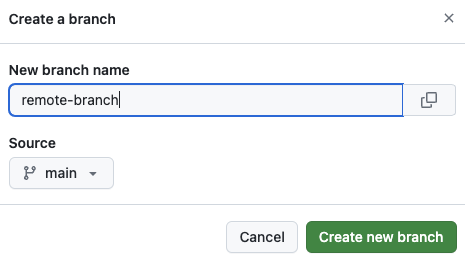
\includegraphics{img/github-create-new-branch.png}
\end{center}

After that, you can use \texttt{kart\ pull} to pull information from the
remote repository, you should see something like this:

\begin{Shaded}
\begin{Highlighting}[]
\ExtensionTok{kart}\NormalTok{ pull}

 \ExtensionTok{*}\NormalTok{ [new branch]      remote{-}branch }\AttributeTok{{-}}\OperatorTok{\textgreater{}}\NormalTok{ origin/remote{-}branch}
\ExtensionTok{Merging}\NormalTok{ 890e245 into feature}
\ExtensionTok{Already}\NormalTok{ up to date}
\end{Highlighting}
\end{Shaded}

And running \texttt{kart\ branch\ -a} confirm that everything has been
updated correctly:

\begin{Shaded}
\begin{Highlighting}[]
\ExtensionTok{kart}\NormalTok{ branch }\AttributeTok{{-}a}

\ExtensionTok{*}\NormalTok{ feature}
  \ExtensionTok{main}
  \ExtensionTok{remotes/origin/feature}
  \ExtensionTok{remotes/origin/main}
  \ExtensionTok{remotes/origin/remote{-}branch}
\end{Highlighting}
\end{Shaded}

You can see from the above that the \texttt{remote-branch} is only
existing on the remote repository, not in your machine (there are two
entries for any branch except this one). If you want to work on this
branch, you can simply run \texttt{kart\ switch\ remote-branch}, and the
new branch will be automatically linked to the remote one.

\begin{Shaded}
\begin{Highlighting}[]
\ExtensionTok{kart}\NormalTok{ switch remote{-}branch}

\ExtensionTok{Creating}\NormalTok{ new branch }\StringTok{\textquotesingle{}remote{-}branch\textquotesingle{}}\NormalTok{ to track }\StringTok{\textquotesingle{}origin/remote{-}branch\textquotesingle{}}\NormalTok{...}
\end{Highlighting}
\end{Shaded}

\subparagraph{Delete local and remote
branches}\label{delete-local-and-remote-branches}

If you want to delete a local branch that you already pushed on remote,
you need some few additional steps.

\begin{enumerate}
\def\labelenumi{\arabic{enumi}.}
\tightlist
\item
  Delete your local development branch with
  \texttt{kart\ branch\ -d\ remote-branch}, replacing remote-branch with
  the actual name of your branch. Note that you cannot delete the branch
  you are currently on, so you will need to switch to another branch in
  order to delete it.
\item
  Use \texttt{kart\ push\ origin\ -\/-delete\ remote-branch}, replacing
  remote-branch with the actual name of your development branch.
\item
  If you deleted the branch on the remote forge/github before deleting
  it locally on your machine, the previous command will fail. You will
  need to update the remote information locally using
  \texttt{kart\ fetch\ -\/-prune}, which will usually tell you that the
  remote branch is deleted. Then you can proceed to delete the local
  branch as in the step \texttt{1}.
\end{enumerate}

\begin{Shaded}
\begin{Highlighting}[]
\ExtensionTok{kart}\NormalTok{ branch }\AttributeTok{{-}d}\NormalTok{ remote{-}branch}

\ExtensionTok{Deleted}\NormalTok{ branch remote{-}branch }\ErrorTok{(}\ExtensionTok{was}\NormalTok{ 890e245}\KeywordTok{)}\BuiltInTok{.}

\ExtensionTok{kart}\NormalTok{ push origin }\AttributeTok{{-}{-}delete}\NormalTok{ remote{-}branch}

\ExtensionTok{To}\NormalTok{ https://github.com/yourusername/kart{-}tutorial.git}
 \ExtensionTok{{-}} \PreprocessorTok{[}\SpecialStringTok{deleted}\PreprocessorTok{]}\NormalTok{         remote{-}branch}
\end{Highlighting}
\end{Shaded}

You can go on your forge to see that the changes have been reflected
over there too.

\section{Tips}\label{tips}

\subsection{\texorpdfstring{\textbf{Selective import
tables}}{Selective import tables}}\label{selective-import-tables}

\subsection{\texorpdfstring{\textbf{Rename data on
import}}{Rename data on import}}\label{rename-data-on-import}

\subsection{\texorpdfstring{\textbf{Create data from QGIS and start
version them with
kart}}{Create data from QGIS and start version them with kart}}\label{create-data-from-qgis-and-start-version-them-with-kart}

In QGIS, new layers can be safely added to the kart geopackage using the
\texttt{New\ Geopackage\ Layer} button. However, this layer will not be
automatically tracked by kart, which needs to be told manually about
their existence:

Since version \texttt{0.12.3} (2023-04-26) kart provides the command
\texttt{kart\ add-dataset}. This command tells kart to track layers that
are present in the geopackage, but that were not imported through
\texttt{kart\ import}. This command is mentioned in a
\href{https://github.com/koordinates/kart/issues/830}{github issue}, but
it is not documented yet in the official documentation at the time of
writing (2024-04-01), thus we put here a quick reference to document its
existence.

The workflow for creating and start versioning new layers in kart is as
follows:

\begin{enumerate}
\def\labelenumi{\arabic{enumi}.}
\item
  Create a new geopackage layer, either from scratch using the ``New
  Geopackage Layer'' dialog, or through the ``Save as..'' option if you
  have an existing layer already in your project.
\item
  Open the terminal (the \texttt{add-dataset} is still not implemented
  in the kart qgis plugin) and navigate to the directory where your kart
  geopackage is located.
\item
  Check if the layer is indeed present inside the geopackage by running
  \texttt{kart\ status\ -\/-list-untracked-tables}. You should get
  something along the lines of:

\begin{Shaded}
\begin{Highlighting}[]
\ExtensionTok{On}\NormalTok{ branch main}
\ExtensionTok{Your}\NormalTok{ branch is up to date with }\StringTok{\textquotesingle{}origin/main\textquotesingle{}}\NormalTok{.}

\ExtensionTok{Nothing}\NormalTok{ to commit, working copy clean}

\ExtensionTok{Untracked}\NormalTok{ tables:}
  \ExtensionTok{THE}\NormalTok{ UNTRACKED LAYERS}
\end{Highlighting}
\end{Shaded}
\end{enumerate}

NB: if you don't see any untracked layers, make sure you created/saved
the layer in the correct geopackage! NB: kart refers to Vector data as
Table Datasets, which is why in the output you will see ``tables'' and
not ``layers'' (which is more of a GIS concept).

\begin{enumerate}
\def\labelenumi{\arabic{enumi}.}
\setcounter{enumi}{3}
\tightlist
\item
  Run \texttt{kart\ add-dataset\ YOUR-LAYER-NAME} (by replacing
  YOUR-LAYER-NAME with the actual name of the layer), kart will prompt
  for a commit message before starting to track the layer.
\end{enumerate}

Note that this also works for the layer styles when saved to the
geopackage using the dialog option ``Style -\textgreater{} Save as
Default -\textgreater{} Datasource Database'' (from the layer properties
tab). Styles saved in this way are usually saved in a
\texttt{layer\_styles} table inside the geopackage. We can run
\texttt{kart\ add-dataset\ layer\_styles} to track any changes to the
layer styles (check if the layer exists and if it is indeed untracked
first).

\subsubsection{\texorpdfstring{A note on the commit message when running
\texttt{kart\ add-dataset}}{A note on the commit message when running kart add-dataset}}\label{a-note-on-the-commit-message-when-running-kart-add-dataset}

You will be thrown in your terminal text editor (see
Section~\ref{sec-text-editors} to manage the commit message).

\subsubsection{Addendum - layer styles}\label{addendum---layer-styles}

\begin{tcolorbox}[enhanced jigsaw, bottomrule=.15mm, opacitybacktitle=0.6, colback=white, toptitle=1mm, left=2mm, titlerule=0mm, leftrule=.75mm, title=\textcolor{quarto-callout-warning-color}{\faExclamationTriangle}\hspace{0.5em}{Warning}, opacityback=0, colframe=quarto-callout-warning-color-frame, breakable, colbacktitle=quarto-callout-warning-color!10!white, coltitle=black, bottomtitle=1mm, toprule=.15mm, arc=.35mm, rightrule=.15mm]

Note that, at the time of writing (2023-11-15), due to a small
mishandling of layer\_styles schema by QGIS, if your layer name is
longer than 30 characters and your style is named with the same name as
the layer, you will incur into an error when trying to run
\texttt{kart\ add-dataset\ layer\_styles}. As explained
\href{https://github.com/koordinates/kart/issues/873}{in this issue},
this is not a kart bug. We recommend keeping the layer style name (or
the layer names) below 30 characters to avoid issues.

\end{tcolorbox}

\section{Useful Resources}\label{sec-resources}

\begin{itemize}
\tightlist
\item
  \href{https://kartproject.org/}{Kart website}
\end{itemize}

\subsection{Documentation}\label{documentation}

\begin{itemize}
\item
  \href{https://docs.kartproject.org/en/latest/index.html}{Kart
  documentation}
\item
  \href{https://docs.kartproject.org/en/latest/pages/command_reference.html}{Kart
  command reference}
\item
  \href{https://github.com/koordinates/kart-qgis-plugin/blob/main/docs/index.md\#kart-plugin-user-documentation}{Kart
  QGIS plugin documentation}
\end{itemize}

\subsection{Other resources}\label{other-resources}

\subsubsection{Presentations about kart}\label{presentations-about-kart}

\begin{itemize}
\item
  Coup, R. (2022a).
  \href{https://www.youtube.com/watch?v=fAIh6p4rczY}{Kart: An
  introduction to practical data versioning for geospatial}.
\item
  Coup, R. (2022b).
  \href{https://www.youtube.com/watch?v=_7ETwmMlUtY}{Kart: A Practical
  Tool for Versioning Geospatial Data}.
\item
  Coup, R. (2023).
  \href{https://www.youtube.com/watch?v=AxOTE2CCY3s}{2023 QGIS Data
  Versioning with Kart}.
\item
  Olaya, V. (2022).
  \href{https://www.youtube.com/watch?v=aABc3JrgJUY}{Spatial data
  versioning with the Kart QGIS Plugin}.
\end{itemize}

\subsubsection{Guides and tutorials about
Git}\label{guides-and-tutorials-about-git}

\begin{itemize}
\item
  \href{https://dev.to/jitendrachoudhary/understanding-git-a-beginners-guide-to-version-control-with-visuals-5cbf}{Understanding
  Git: A Beginner's Guide to Version Control (With Visuals)}
\item
  \href{https://www.atlassian.com/git}{Getting Git Right}
\item
  \href{https://rogerdudler.github.io/git-guide/index.html}{Git: the
  simple guide}
\item
  \href{https://git-scm.com/doc}{Git Official Documentation with useful
  resources}
\item
  \href{https://git-scm.com/doc/ext}{Other tutorials from the Git
  website}
\end{itemize}

\subsubsection{QGIS}\label{qgis}

\begin{itemize}
\item
  \href{https://qgis.org}{QGIS Website}
\item
  \href{https://docs.qgis.org/latest/en/docs/user_manual/}{QGIS User
  Guide}
\item
  \href{https://docs.qgis.org/3.34/en/docs/training_manual/}{QGIS
  Training Manual}
\item
  \href{https://docs.qgis.org/3.34/en/docs/gentle_gis_introduction/}{A
  Gentle Introduction to QGIS}
\end{itemize}



\end{document}
